\documentclass[a4paper, 12pt]{article}
\usepackage{geometry}
\usepackage{graphicx}
\usepackage{mathtools}
\usepackage{listings}
\usepackage{float}
\usepackage[utf8]{inputenc}
\geometry{margin=1in}

\usepackage{color} %red, green, blue, yellow, cyan, magenta, black, white
\definecolor{mygreen}{RGB}{28,172,0} % color values Red, Green, Blue
\definecolor{mylilas}{RGB}{170,55,241}

\begin{document}

\section{Vergelijkende analyse van discreet equivalent}

\lstset{language=Matlab,%
    %basicstyle=\color{red},
    breaklines=true,%
    morekeywords={matlab2tikz},
    keywordstyle=\color{blue},%
    morekeywords=[2]{1}, keywordstyle=[2]{\color{black}},
    identifierstyle=\color{black},%
    stringstyle=\color{mylilas},
    commentstyle=\color{mygreen},%
    showstringspaces=false,%without this there will be a symbol in the places where there is a space
    numbers=left,%
    numberstyle={\tiny \color{black}},% size of the numbers
    numbersep=9pt, % this defines how far the numbers are from the text
    emph=[1]{for,end,break},emphstyle=[1]\color{red}, %some words to emphasise
    %emph=[2]{word1,word2}, emphstyle=[2]{style},    
}
\begin{lstlisting}
ts = 0.1;
c1 = tf([1], [1 1])
d1 = tf([ts], [1 -1+ts], ts)
d2 = tf([ts/(ts+1) 0], [1 -1/(ts+1)], ts)
d3 = tf([ts ts], [ts+2 -2+ts], ts)
d4 = tf([1-exp(-ts) +1-exp(-ts)], [2 -2*exp(-ts)], ts)
d5 = tf([1-exp(-ts)], [1 -exp(-ts)], ts)

step(c1, d1, d2, d3, d4, d5)
legend('c1', 'd1', 'd2', 'd3', 'd4', 'd5')
\end{lstlisting}

Dit is de broncode van het matlab script dat de stapresponsies geeft voor verschillende discrete equivalenten.\\
Deze code geeft volgend resultaat.

\begin{figure}[!h]
	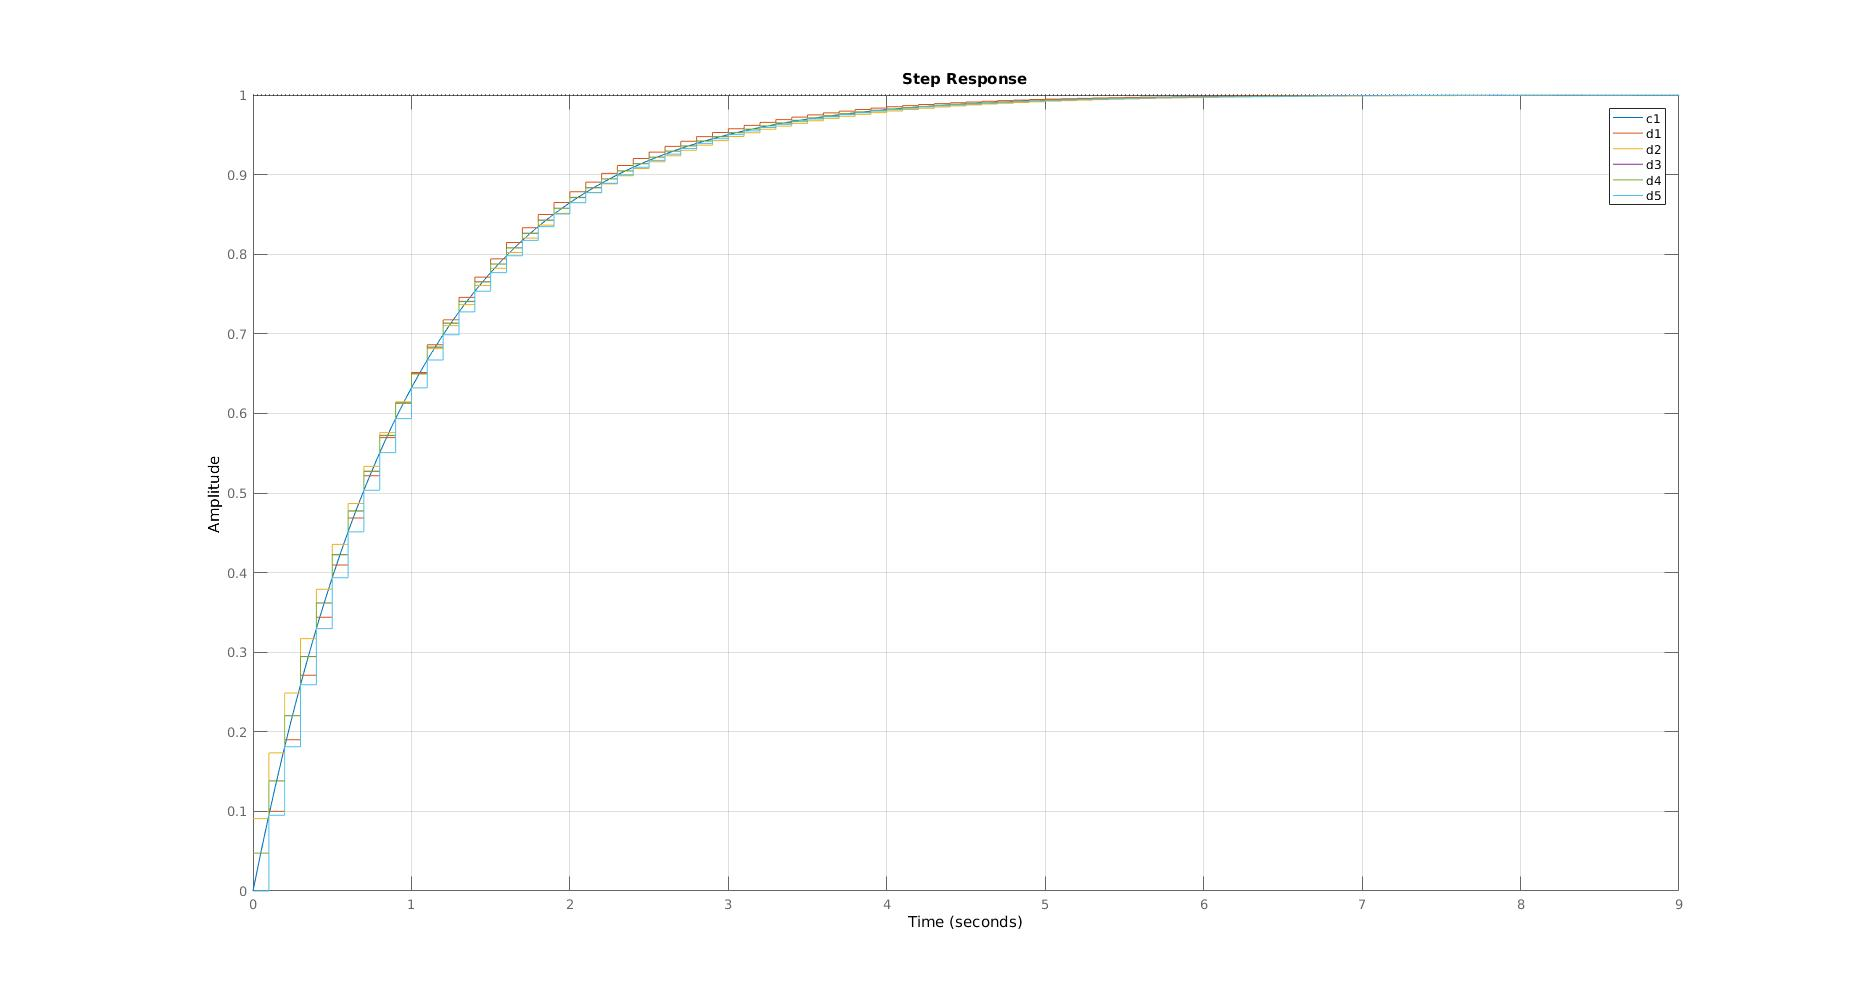
\includegraphics[width=1\linewidth]{Labo3_step_response.jpg}
	\caption{Stepresponse van het continu en de 5 discrete systemen}
	\label{fig:Labo3_step_response}
\end{figure}

Op deze figuur zien we niet veel. Wat wel wel zien is dat ruw gezien alle discrete equivalenten het continu systeem lijken te volgen.\\
Maar we gaan deze figuur toch in wat meer detail bekijken.

\begin{figure}[H]
	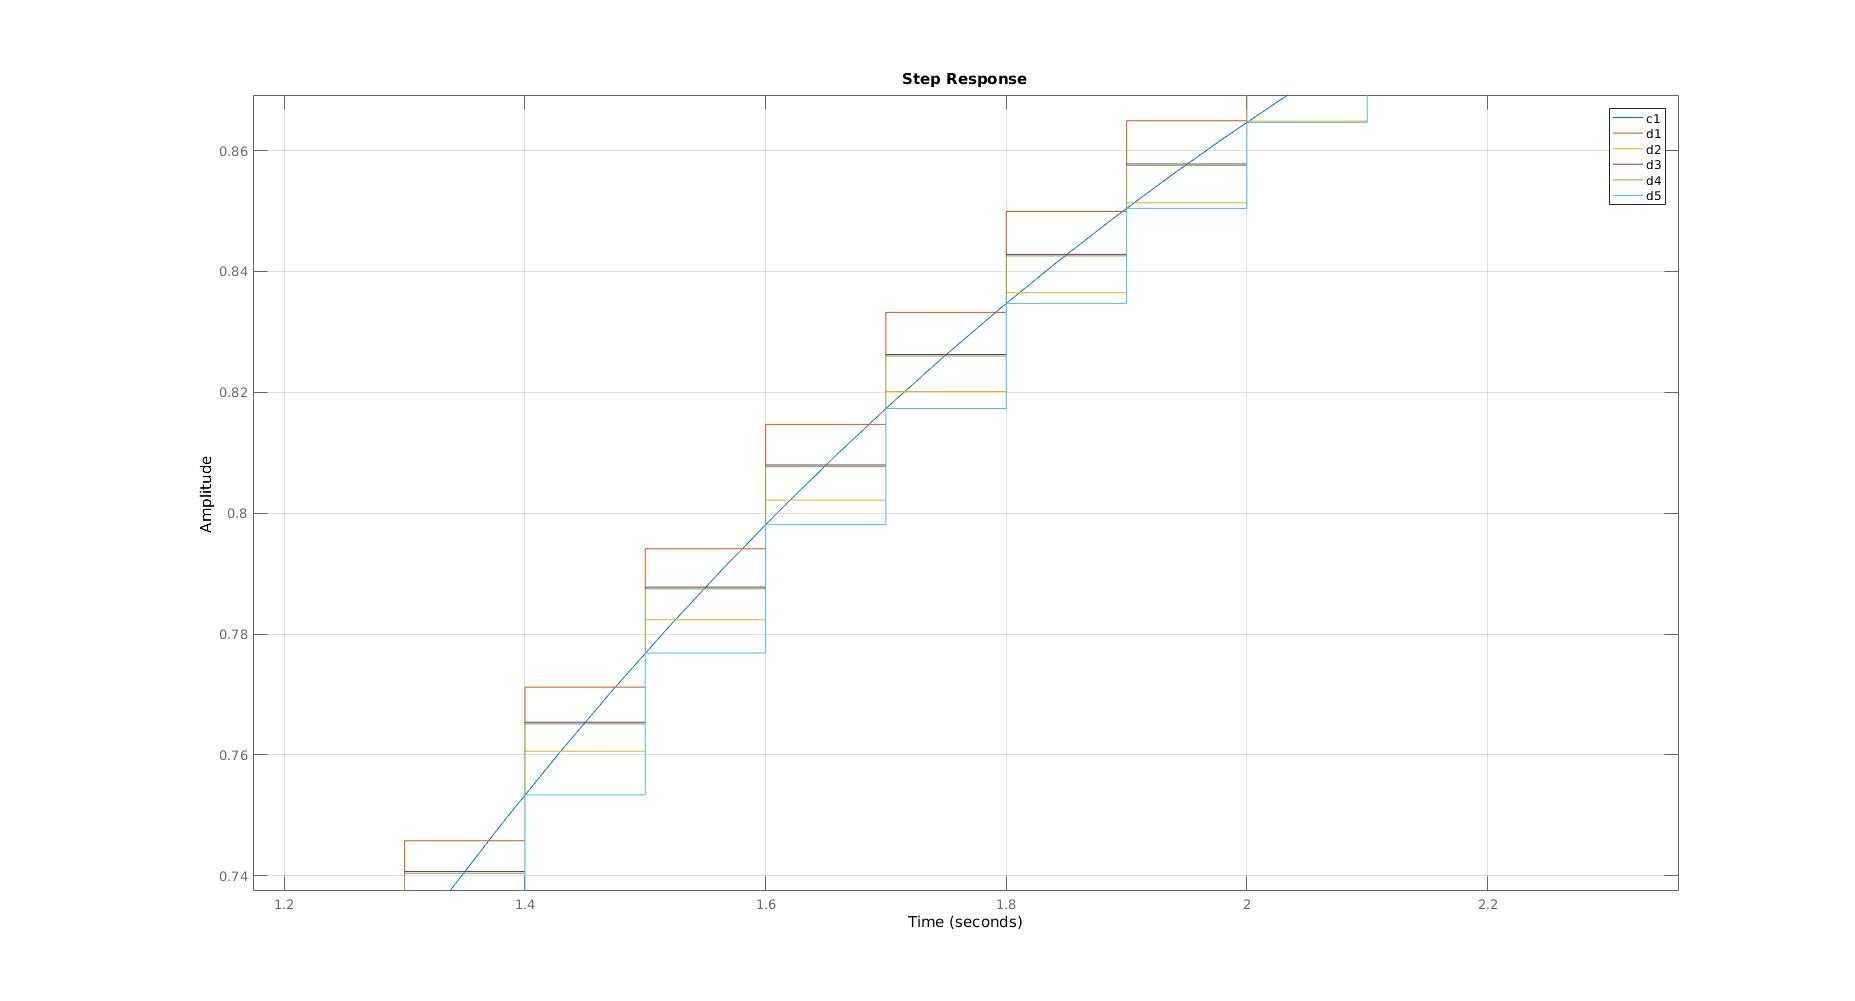
\includegraphics[width=1\linewidth]{Labo3_step_response2.jpg}
	\caption{ingezoomde stepresponse}
	\label{fig:Labo3_step_response_zoom}
\end{figure}

Figuur \ref{fig:Labo3_step_response_zoom} geeft een beter beeld op figuur \ref{fig:Labo3_step_response}. Met deze figuur zullen we dan ook een paar vaststellingen kunnen doen. \\

\underline{Welke 2 discrete equivalenten zijn bijna identiek?}\\
Als we goed naar de figuur kijken kunnen we zien dat systeem d3 en d4 bijna op elkaar vallen, en dus ook bij identiek zijn. Dit zijn respectievelijk het systeem met de Trapeziumregel en het systeem met de Nulpunten/polen-transformatie.\\

\underline{Welke discrete TF levert exacte digitale waarden op; dit is identiek aan de continue waarden?}\\
De systemen die exacte digitale waarden geven zijn ook weer de trapeziumregel en de nulpunten/polen-transformatie, omdat deze systemen evenveel punten boven als onder het continu systeem hebben liggen.\\

\underline{Welke twee discrete equivalenten geven een slechte benadering?}\\
De systemen die het meest aan de buitenkant liggen en dus de slechtste benadering geven zijn: d1 en d5. Deze systemen zijn respectievelijk het systeem met de voorwaartse integratieregel en het systeem met het Houdequivalent. bijkomend aan de voorwaartse integratieregel kunnen we ook stellen dat de achterwaartse integratieregel, d2 in dit geval, een even slechte benadering geeft als de voorwaartse integratieregel. \\

\newpage

\begin{lstlisting}
c1 = tf([1], [1 1])
d6 = tf([1-exp(-1)], [1 -exp(-1)], 1)

[ampl, tijd] = step(d6);
figure, stem(tijd, ampl);
hold on, step(c1)
\end{lstlisting}

\begin{figure}[!h]
	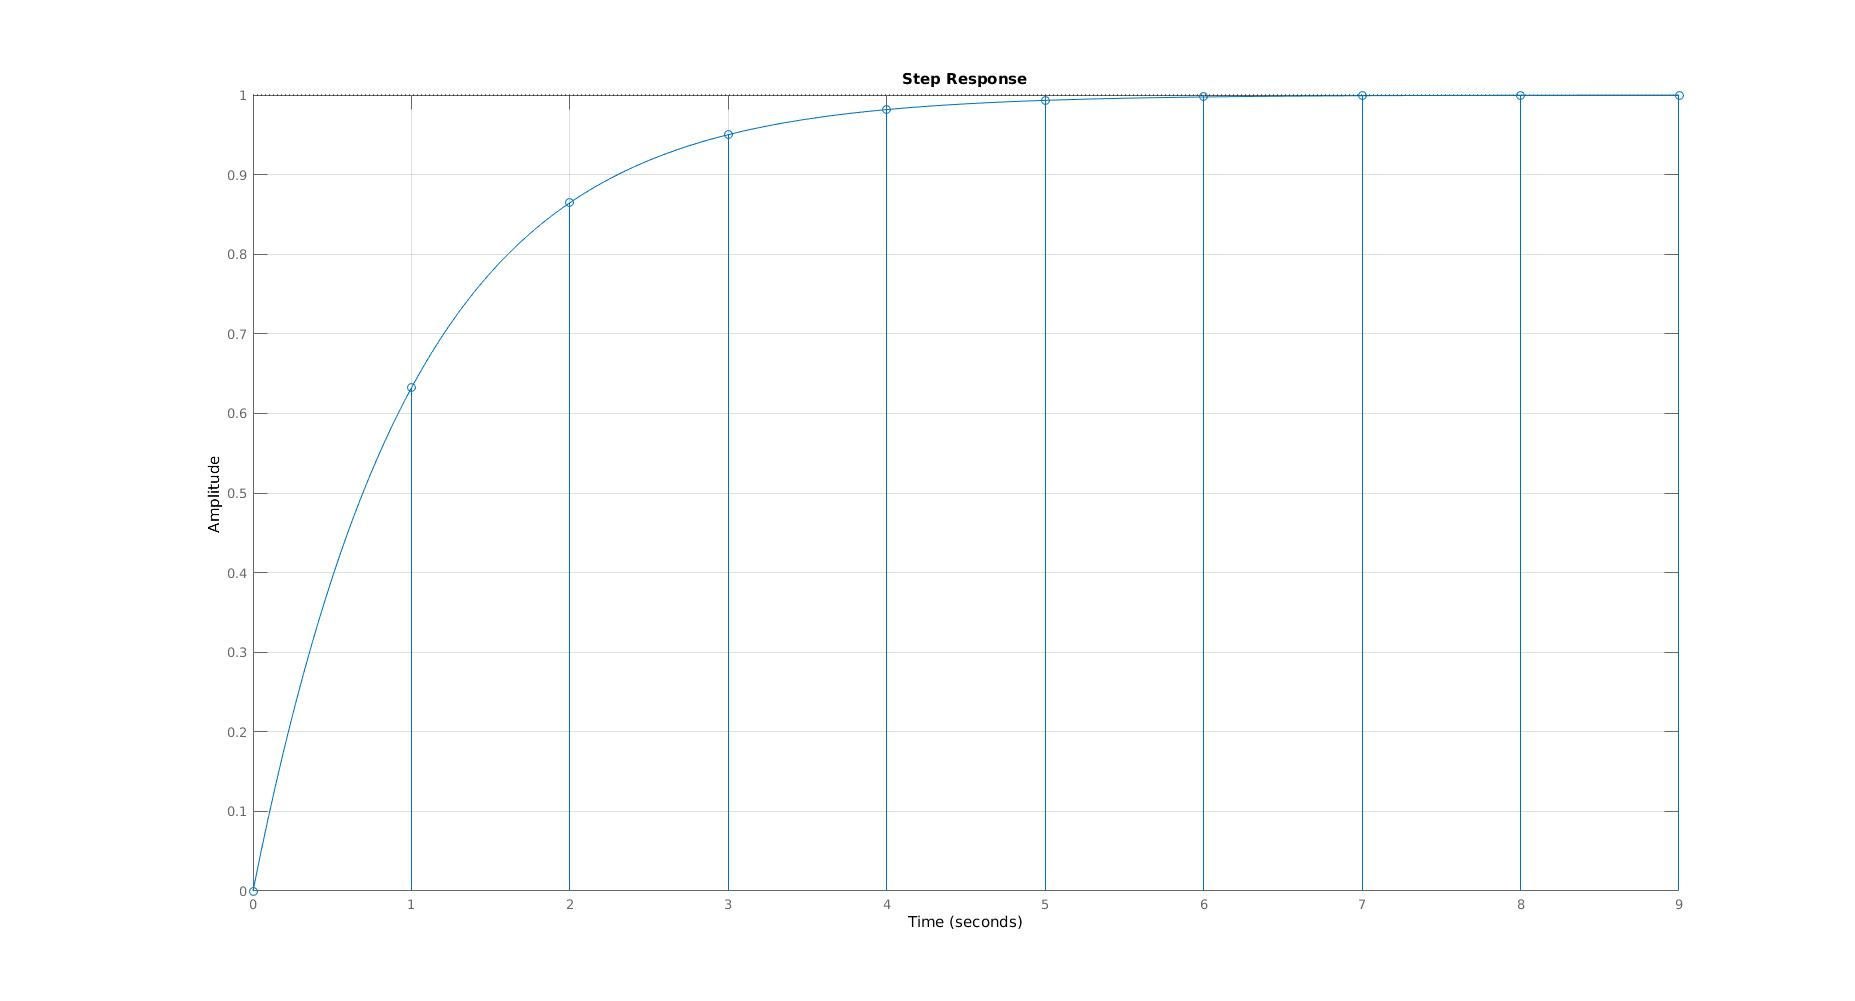
\includegraphics[width=1\linewidth]{Labo3_step_response3.jpg}
	\caption{stepresponse van het continu systeem met het houdequivalent}
	\label{fig:Labo3_step_response2}
\end{figure}

Figuur \ref{fig:Labo3_step_response2} geeft	 continu systeem c1 weer plus het houdequivalent, de horizontale lijnen, voor een sampletijd van 1 seconde, dus een discreet systeem. Zoals te zien is op de figuur vallen de berekende waarden van het houdequivalent perfect samen met het continu systeem, we mogen dus besluiten dat het houdequivalent goed is naar amplitude toe.\\

\begin{lstlisting}
c1 = tf([1], [1 1])
d1 = tf([ts], [1 -1+ts], ts)
d2 = tf([ts/(ts+1) 0], [1 -1/(ts+1)], ts)
d3 = tf([ts ts], [ts+2 -2+ts], ts)
d4 = tf([1-exp(-ts) +1-exp(-ts)], [2 -2*exp(-ts)], ts)
d5 = tf([1-exp(-ts)], [1 -exp(-ts)], ts)

figure, bode(c1, d1, d2, d3, d4, d5)
legend('c1', 'd1', 'd2', 'd3', 'd4', 'd5')
\end{lstlisting}

\begin{figure}[H]
	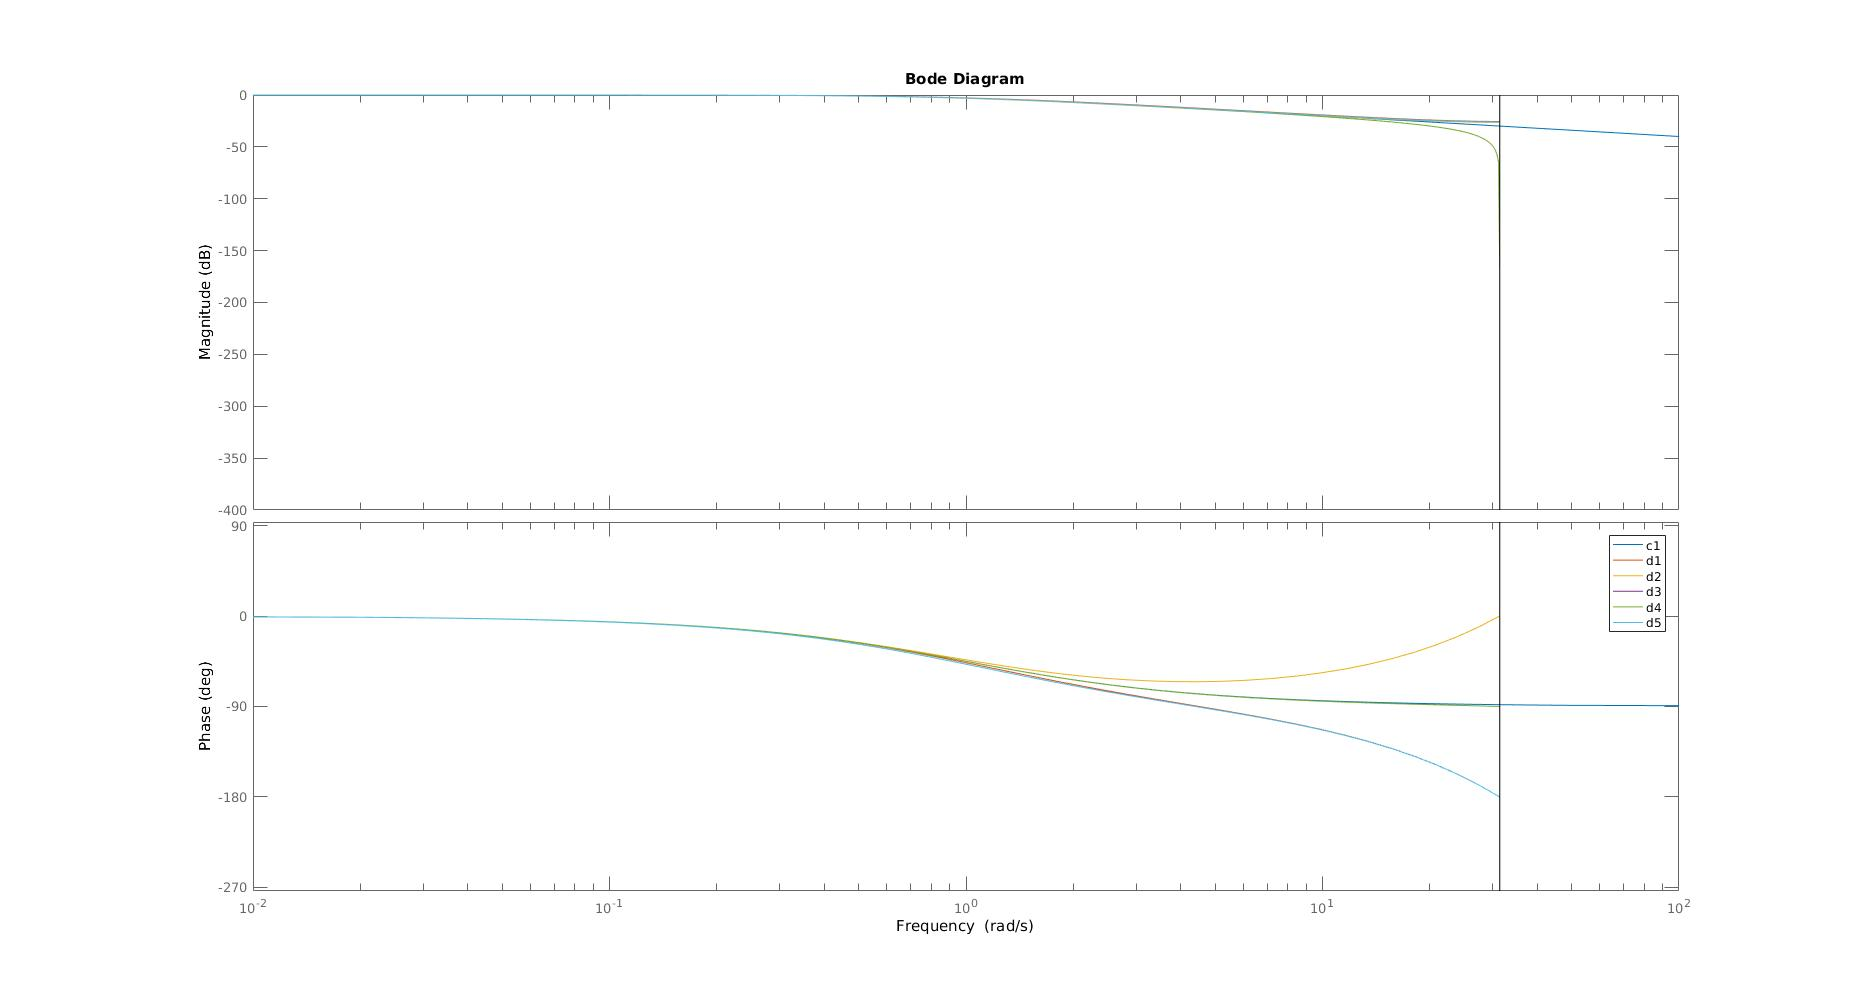
\includegraphics[width=1\linewidth]{Labo3_bode_plot}
	\caption{bode plot van het continu systeem en zijn discrete equivalenten}
\end{figure}

\underline{Tot op welke frequentie is de benadering geldig}\\
De benadering van discrete systemen is geldig tot op de helft van de samplefrequentie. Dit is te danken aan het criterium van Nyquist-Shannon. \\
$t_s = 0,1s \rightarrow f = 10Hz \rightarrow \omega\textsubscript{s} = 2 * \pi *10Hz = 62,8\frac{rad}{s} \rightarrow \omega\textsubscript{max} = \frac{\omega\textsubscript{s}}{2} = 31,4\frac{rad}{s}$ \\

\underline{Welke equivalenten geven een goede benadering (in amplitude en/of in fase) en welke niet?}\\
De systemen die de beste benadering geven zijn toch weer de trapeziumregel en de nulpunten/polen-transformatie. De beste van deze 2 discrete equivalenten is dan nog de trapeziumregel omdat deze voor zowel amplitude- als faseverloop het continu systeem vrij goed benadert. De nulpunten/polen-transformatie wijkt in het amplitudeverloop af tegenover het continu systeem. \\
De systemen die de slechtste benadering geven zijn de 2 integratieregels en het houdequivalent. Deze systemen hebben wel ongeveer hetzelfde amplitudeverloop maar wijken veel af in het faseverloop bij hogere frequenties.

\section{Continu naar discreet}

\subsection{Bepaal de werking van deze functie (c2d) m.b.v. de help-functie}

$>>$ help c2d

\begin{lstlisting}
	c2d  Converts continuous-time dynamic system to discrete time.
 
    SYSD = c2d(SYSC,TS,METHOD) computes a discrete-time model SYSD with 
    sample time TS that approximates the continuous-time model SYSC.
    The string METHOD selects the discretization method among the following:
       'zoh'       Zero-order hold on the inputs
       'foh'       Linear interpolation of inputs
       'impulse'   Impulse-invariant discretization
       'tustin'    Bilinear (Tustin) approximation.
       'matched'   Matched pole-zero method (for SISO systems only).
    The default is 'zoh' when METHOD is omitted. The sample time TS should 
    be specified in the time units of SYSC (see "TimeUnit" property).
 
    c2d(SYSC,TS,OPTIONS) gives access to additional discretization options. 
    Use C2DOPTIONS to create and configure the option set OPTIONS. For 
    example, you can specify a prewarping frequency for the Tustin method by:
       opt = c2dOptions('Method','tustin','PrewarpFrequency',.5);
       sysd = c2d(sysc,.1,opt);
 
    For state-space models,
       [SYSD,G] = c2d(SYSC,Ts,METHOD)
    also returns the matrix G mapping the states xc(t) of SYSC to the states 
    xd[k] of SYSD:
       xd[k] = G * [xc(k*Ts) ; u[k]]
    Given an initial condition x0 for SYSC and an initial input value u0=u(0), 
    the equivalent initial condition for SYSD is (assuming u(t)=0 for t<0):
       xd[0] = G * [x0;u0] .
\end{lstlisting}

\begin{table}[!h]
\centering
\resizebox{\columnwidth}{!}{
	\begin{tabular}{p{0.2\linewidth} p{0.1\linewidth} p{0.7\linewidth}}
	zoh & = & nulde orde houdequivalent\\
	foh & = & nulpunten/polen-transformatie \\
	tustin & = & trapzium transformatie voor 1ste orde systeem \\
	matched & = & houdequivalent\\
	\end{tabular} 
}
\end{table}

\begin{lstlisting}
ts = 0.1;
c1 = tf([1], [1 1])

d15 = c2d(c1, ts, 'zoh')
d16 = c2d(c1, ts, 'foh')
d17 = c2d(c1, ts, 'matched')

step(c1, d15, d16, d17)
\end{lstlisting}

\begin{figure}[!h]
	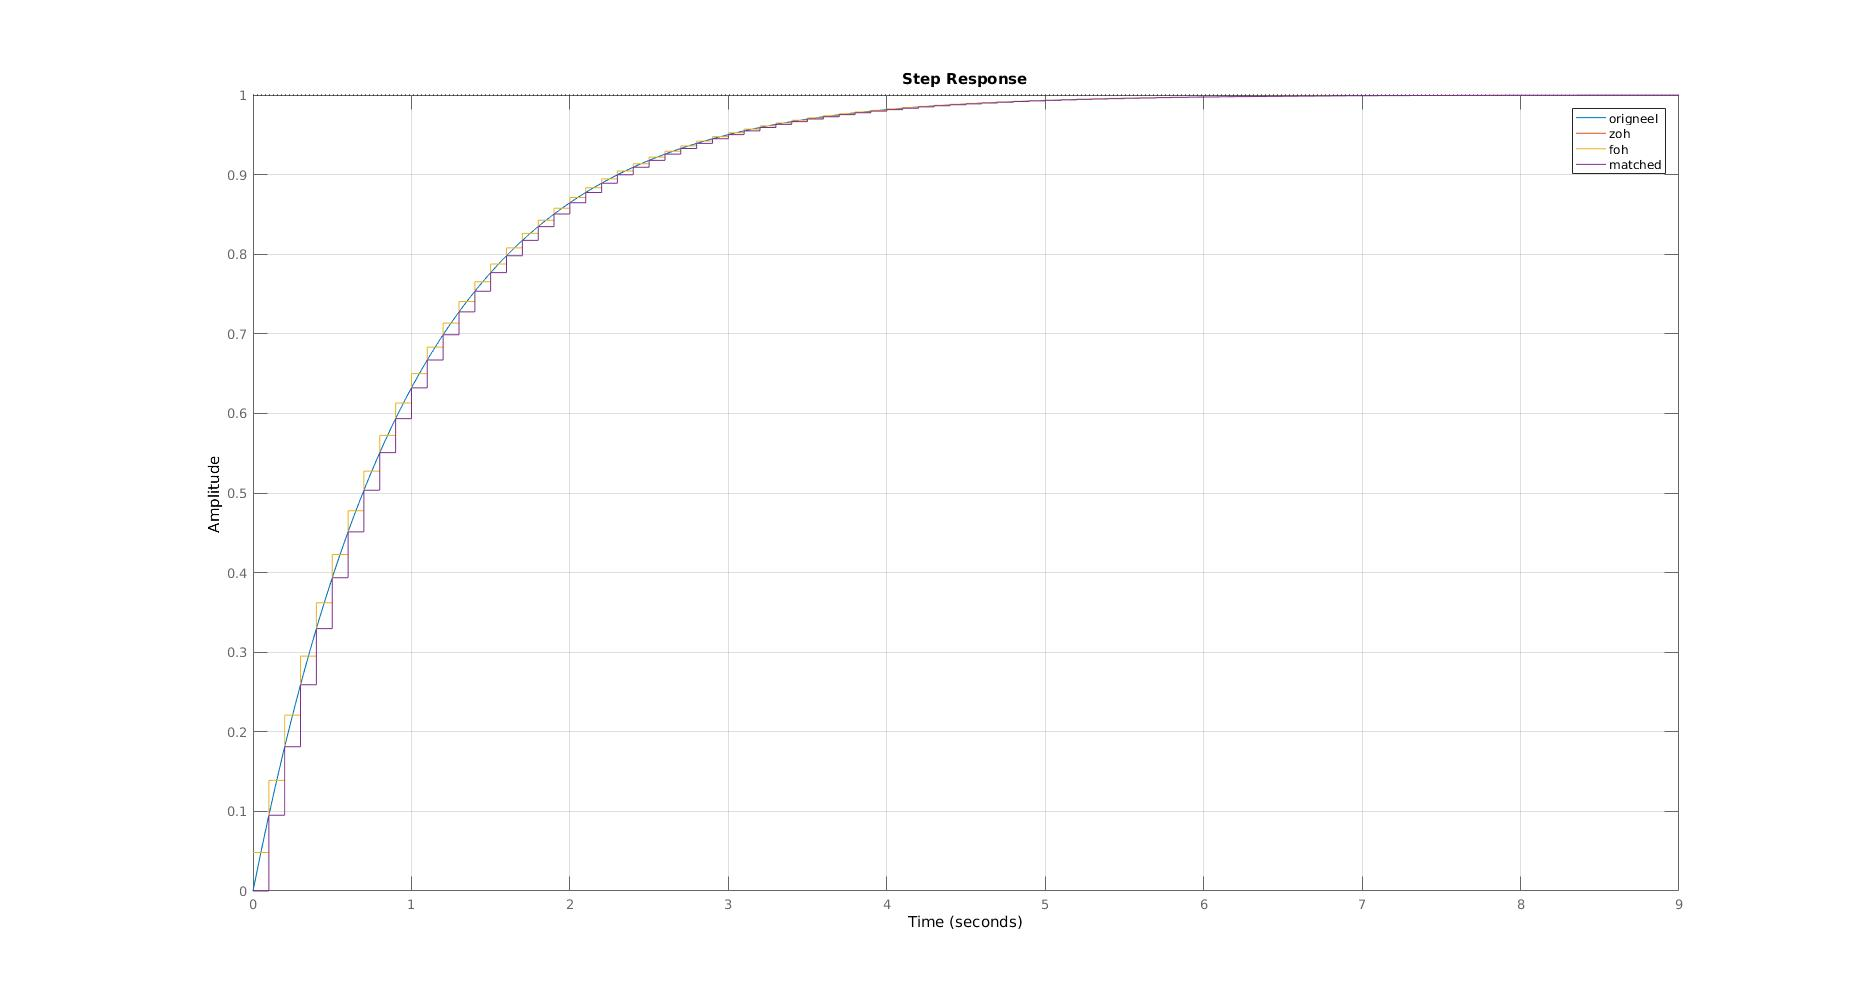
\includegraphics[width=1\linewidth]{Labo3_c2d_stepresponse.jpg}
	\caption{step response van de c2d methodes en het continu systeem}
	\label{labo3_step_response3}
\end{figure}

\begin{figure}[!h]
	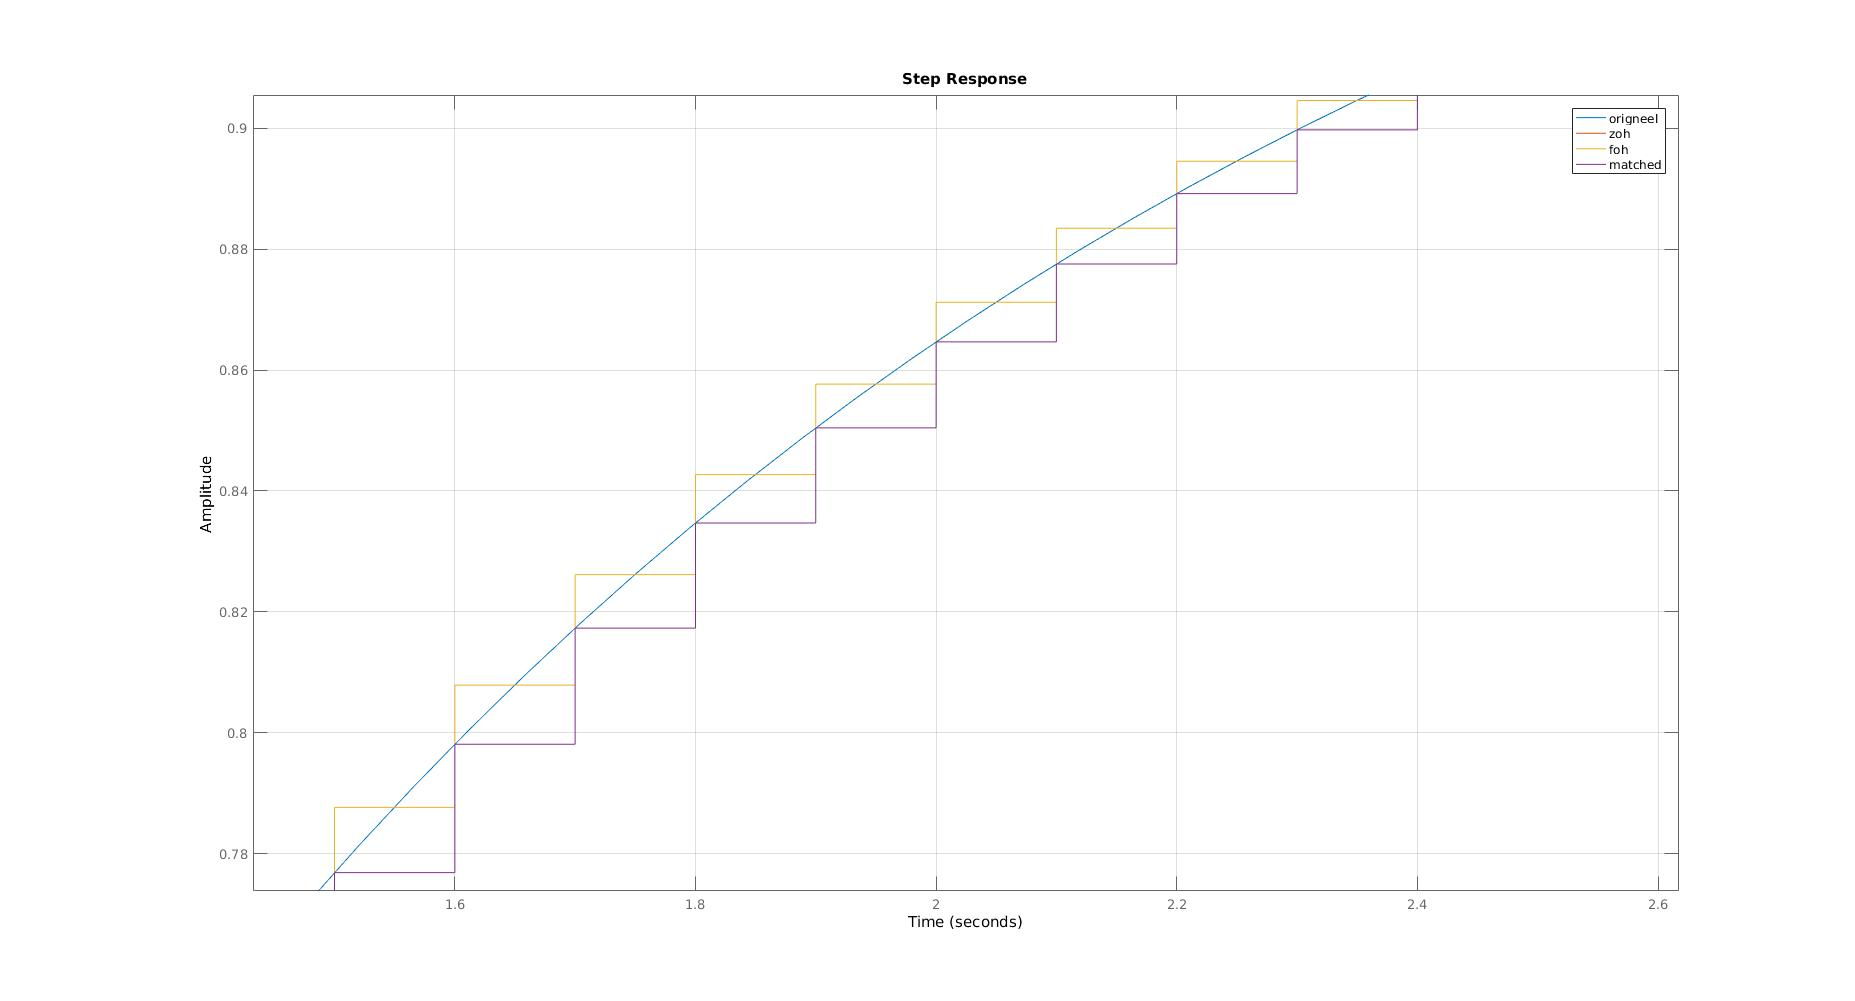
\includegraphics[width=1\linewidth]{Labo3_c2d_stepresponse2.jpg}
	\caption{ingezoomde versie van de step response van de c2d methodes en het continu systeem}
	\label{labo3_step_response4}
\end{figure}

In figuur \ref{labo3_step_response3} en \ref{labo3_step_response4} is de stap response van de c2d functies 'zoh', 'foh' en 'matched' te zien. Hier kunnen we ook in zien dat d16 de nulpunten/polen-transformatie is en de andere 2 (die moeilijk te onderscheiden zijn omdat zo over elkaar vallen) het houdequivalent zijn.

\newpage

\section{Stabiliteitsanalyse}

\subsection{Bereken de marginaliteitsgrens (K\_marg)}

\begin{lstlisting}
ts = 0.040;
G = tf([ts], [1 -1], ts);
H = tf([1], [1 0], ts);
openlus = G*H;

rlocus(openlus)
K = margin(openlus)
\end{lstlisting}

Deze code geeft als resultaat een nulpunten/polen diagram en een waarde voor K\_marg.

\begin{figure}[!h]
	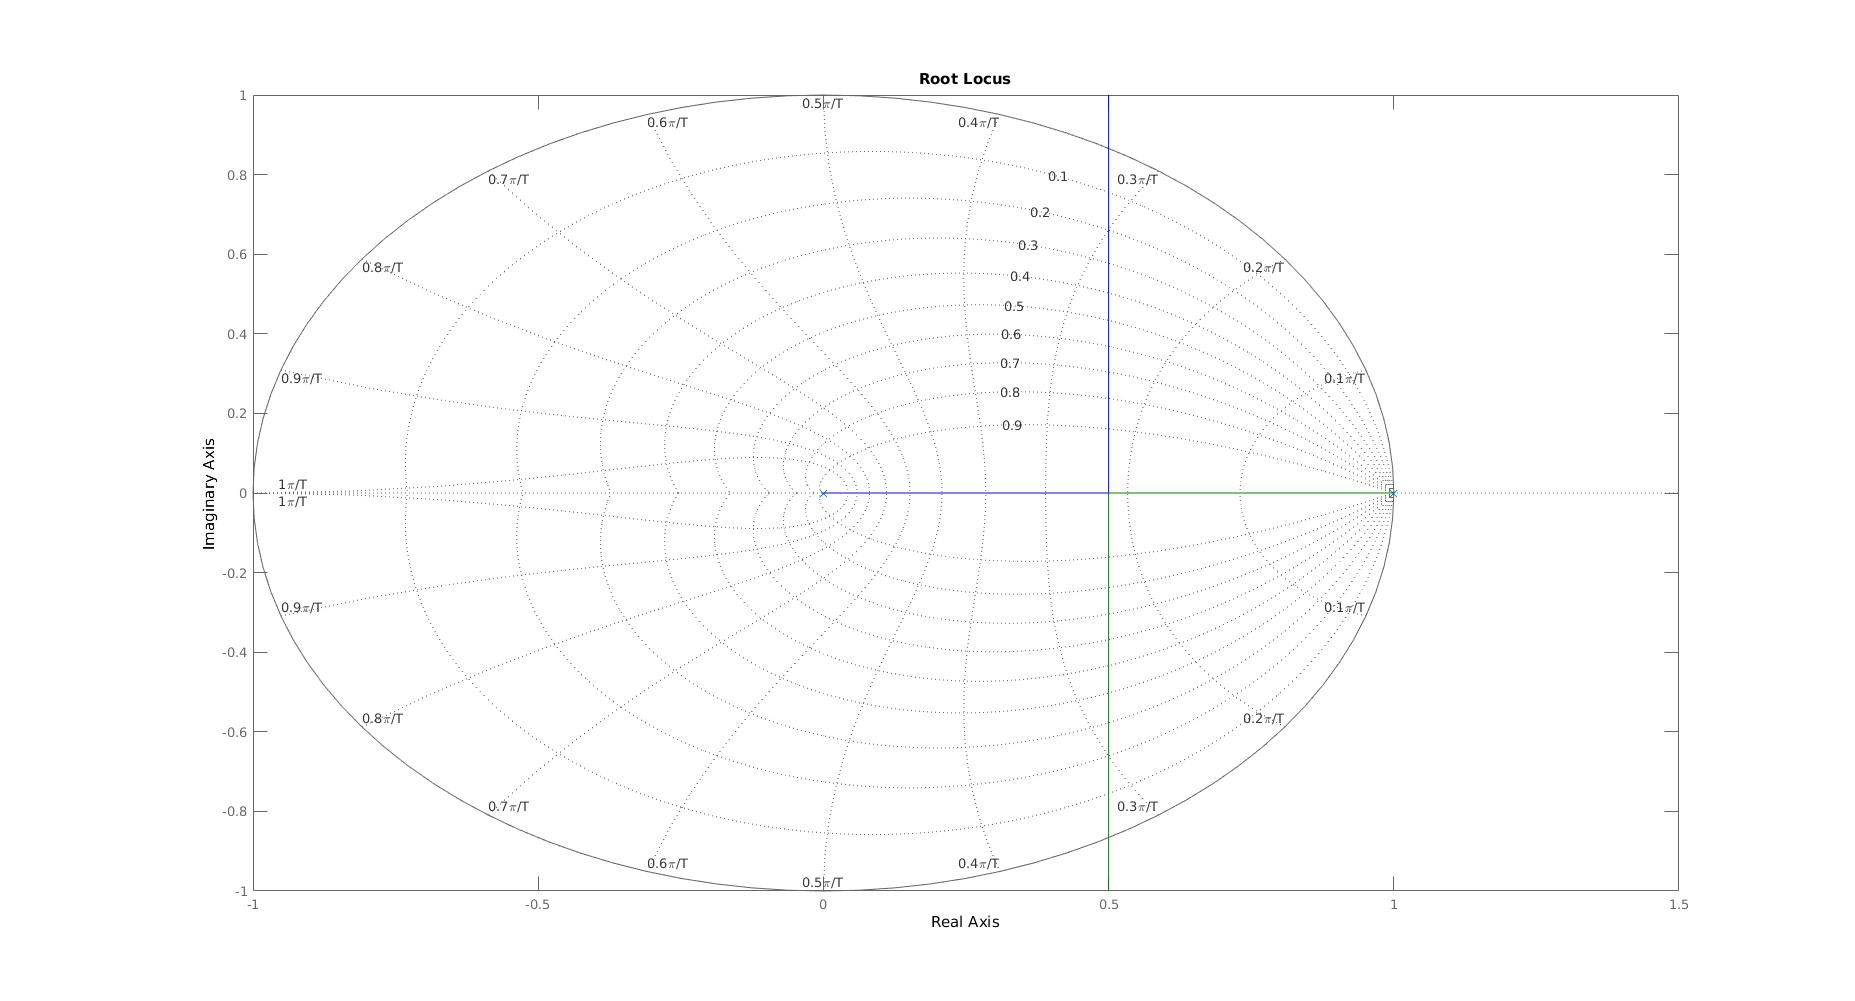
\includegraphics[width=1\linewidth]{Labo3_4_rootlocus.jpg}
	\caption{nulpunten/polen diagram van de open lus}
\end{figure}

Verder geeft matlab via de functie 'margin()' de versterking om een marginaal stabiel systeem te bekomen. In dit geval is K\textsubscript{marg} = 25.

\newpage

\subsection{Toon de gesloten-lus-stapresponsie voor K\textsubscript{marg} = 25}

We hebben de figuur bewust ingezoomd omdat de figuur anders niet leesbaar was.

\begin{figure}[!h]
	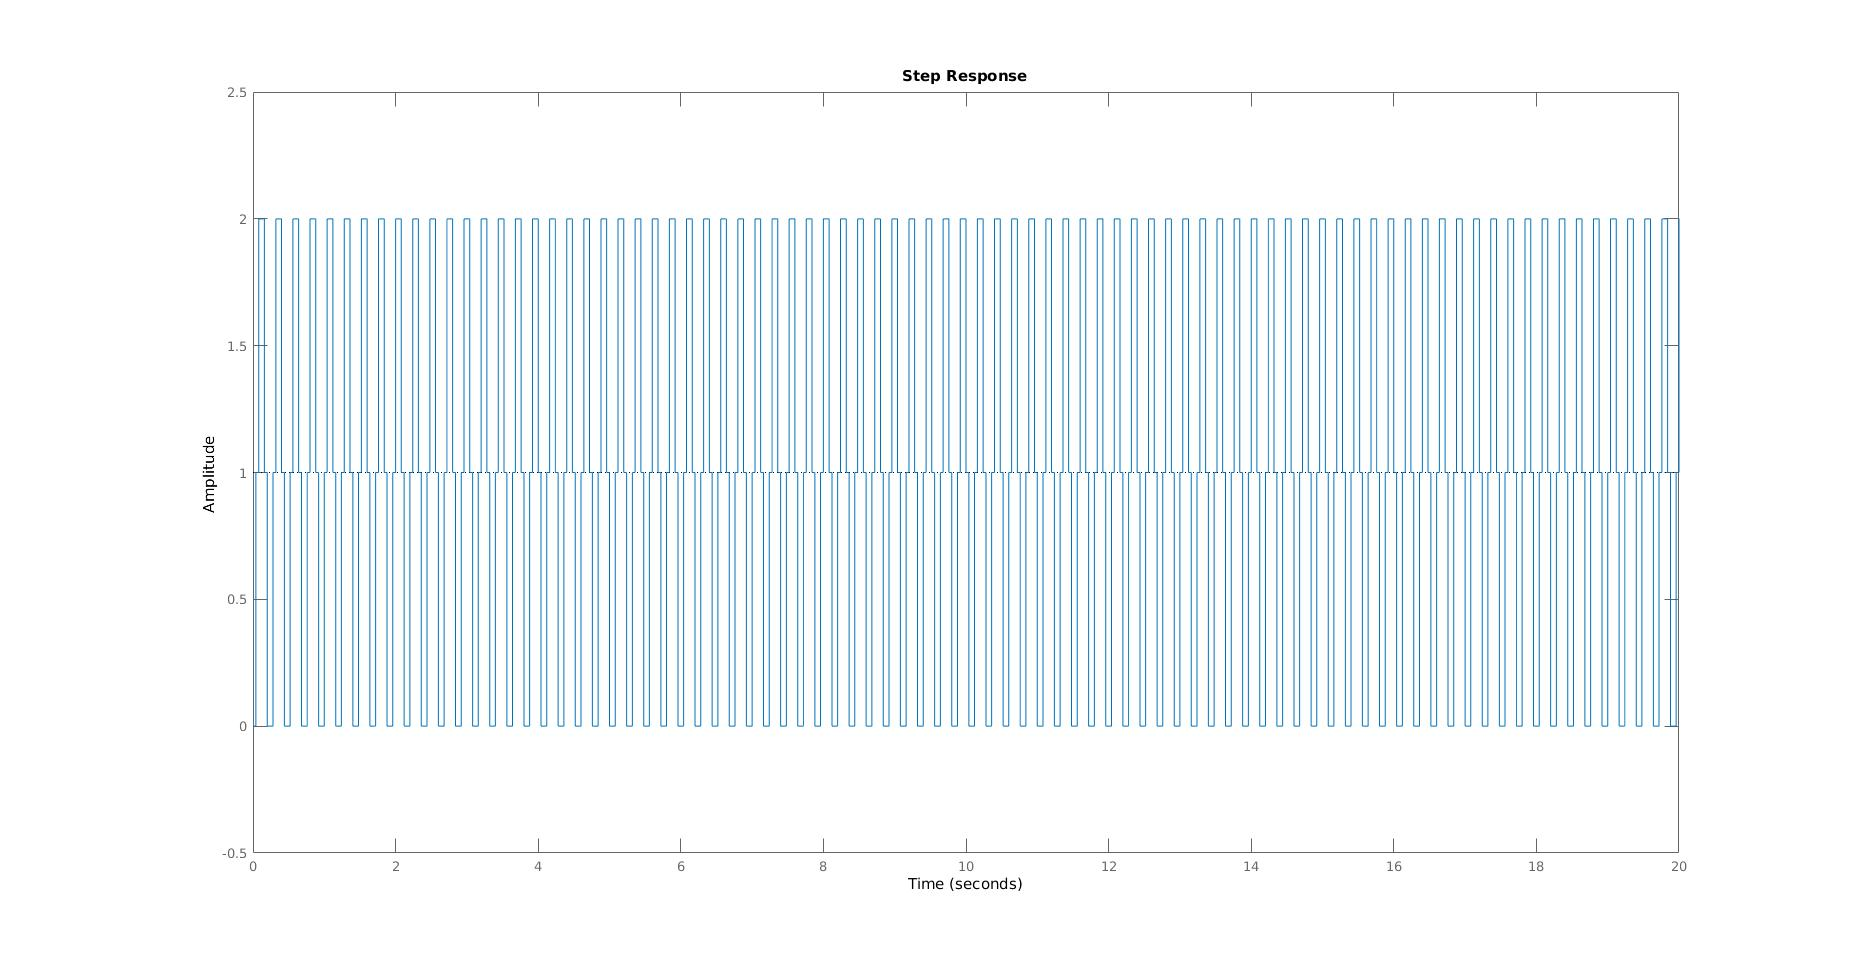
\includegraphics[width=1\linewidth]{Labo3_4_step_response.jpg}
	\caption{stapresponsie van de gesloten lus met k\textsubscript{marg}}
\end{figure}

\subsection{Bereken K voor 4\% doorschot ($\zeta = 0,7$) in de gesloten-lus-stapresponsie en verifieer.}

Voor 4\% doorschot moeten we rekenen met een demping van 0,707.

\begin{figure}[!h]
	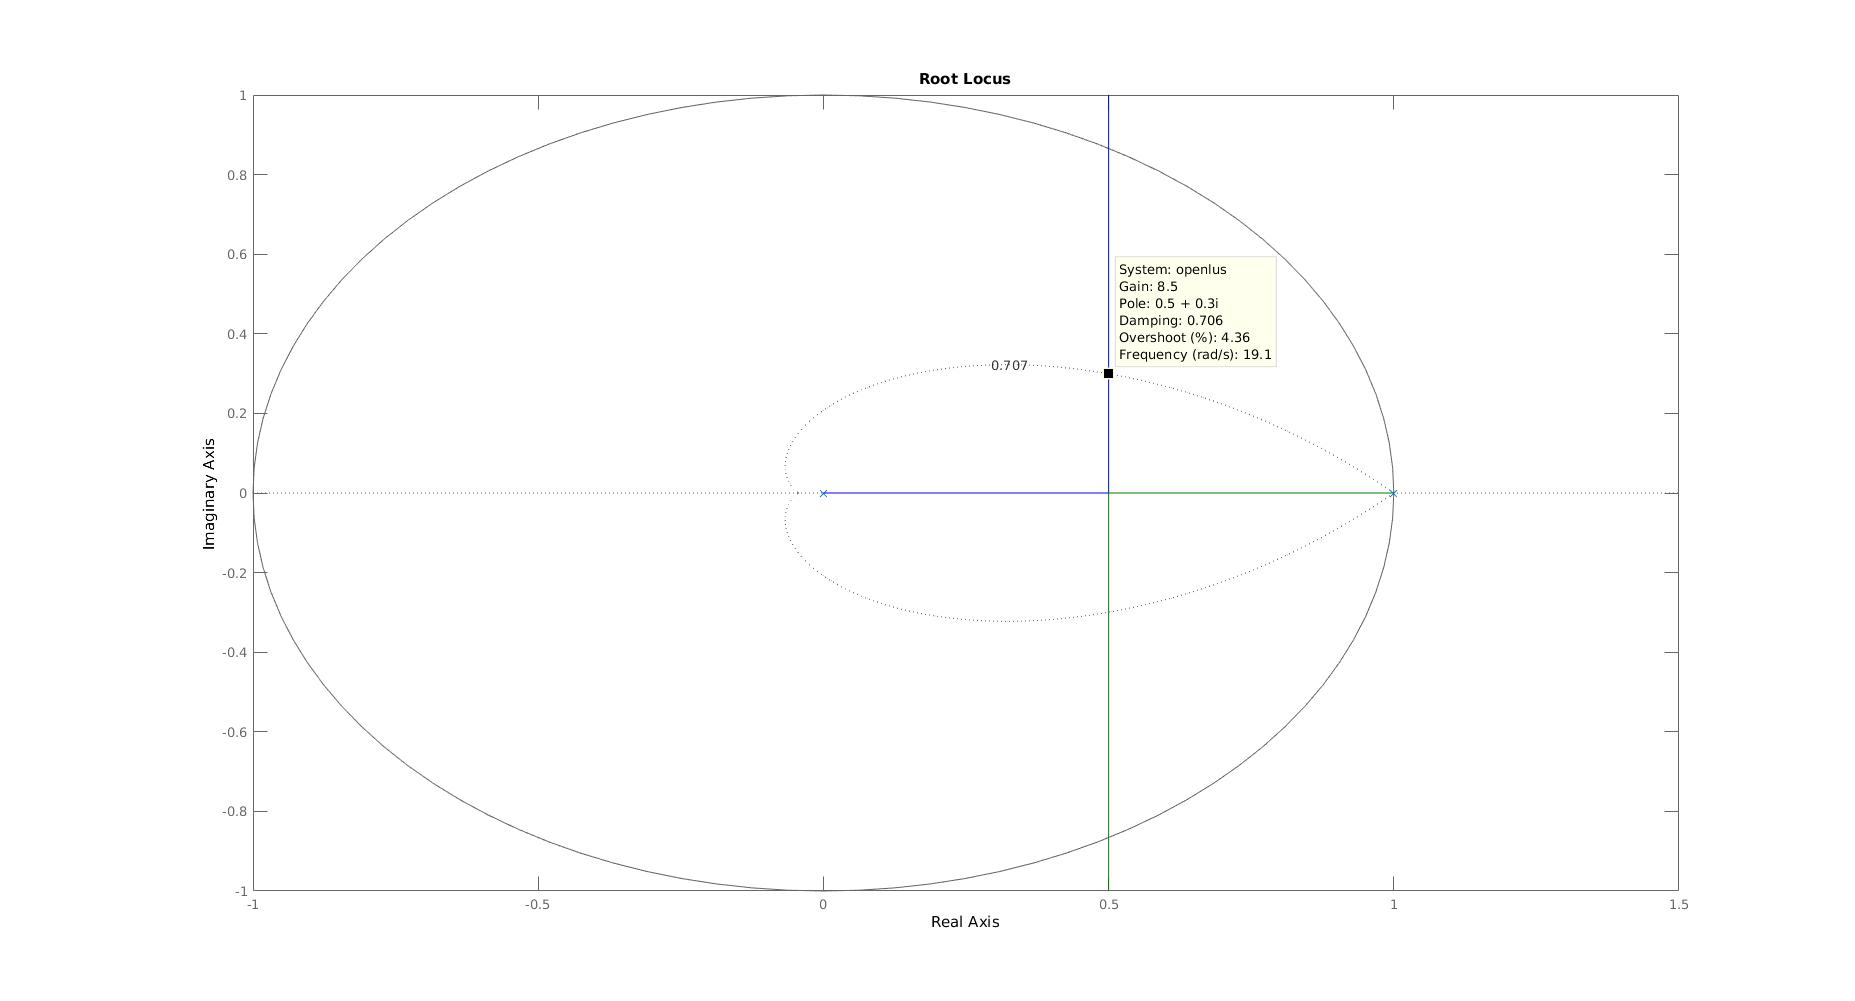
\includegraphics[width=0.9\linewidth]{Labo3_4_rootlocus2.jpg}
	\caption{nulpunten/polen diagram met demping 0,707 aangeduid}
\end{figure}

Uit de figuur kunnen we aflezen dat voor een demping van 0,707 en dus ook doorschot van 4\%, K gelijk is aan 8,5.

\begin{figure}[!h]
	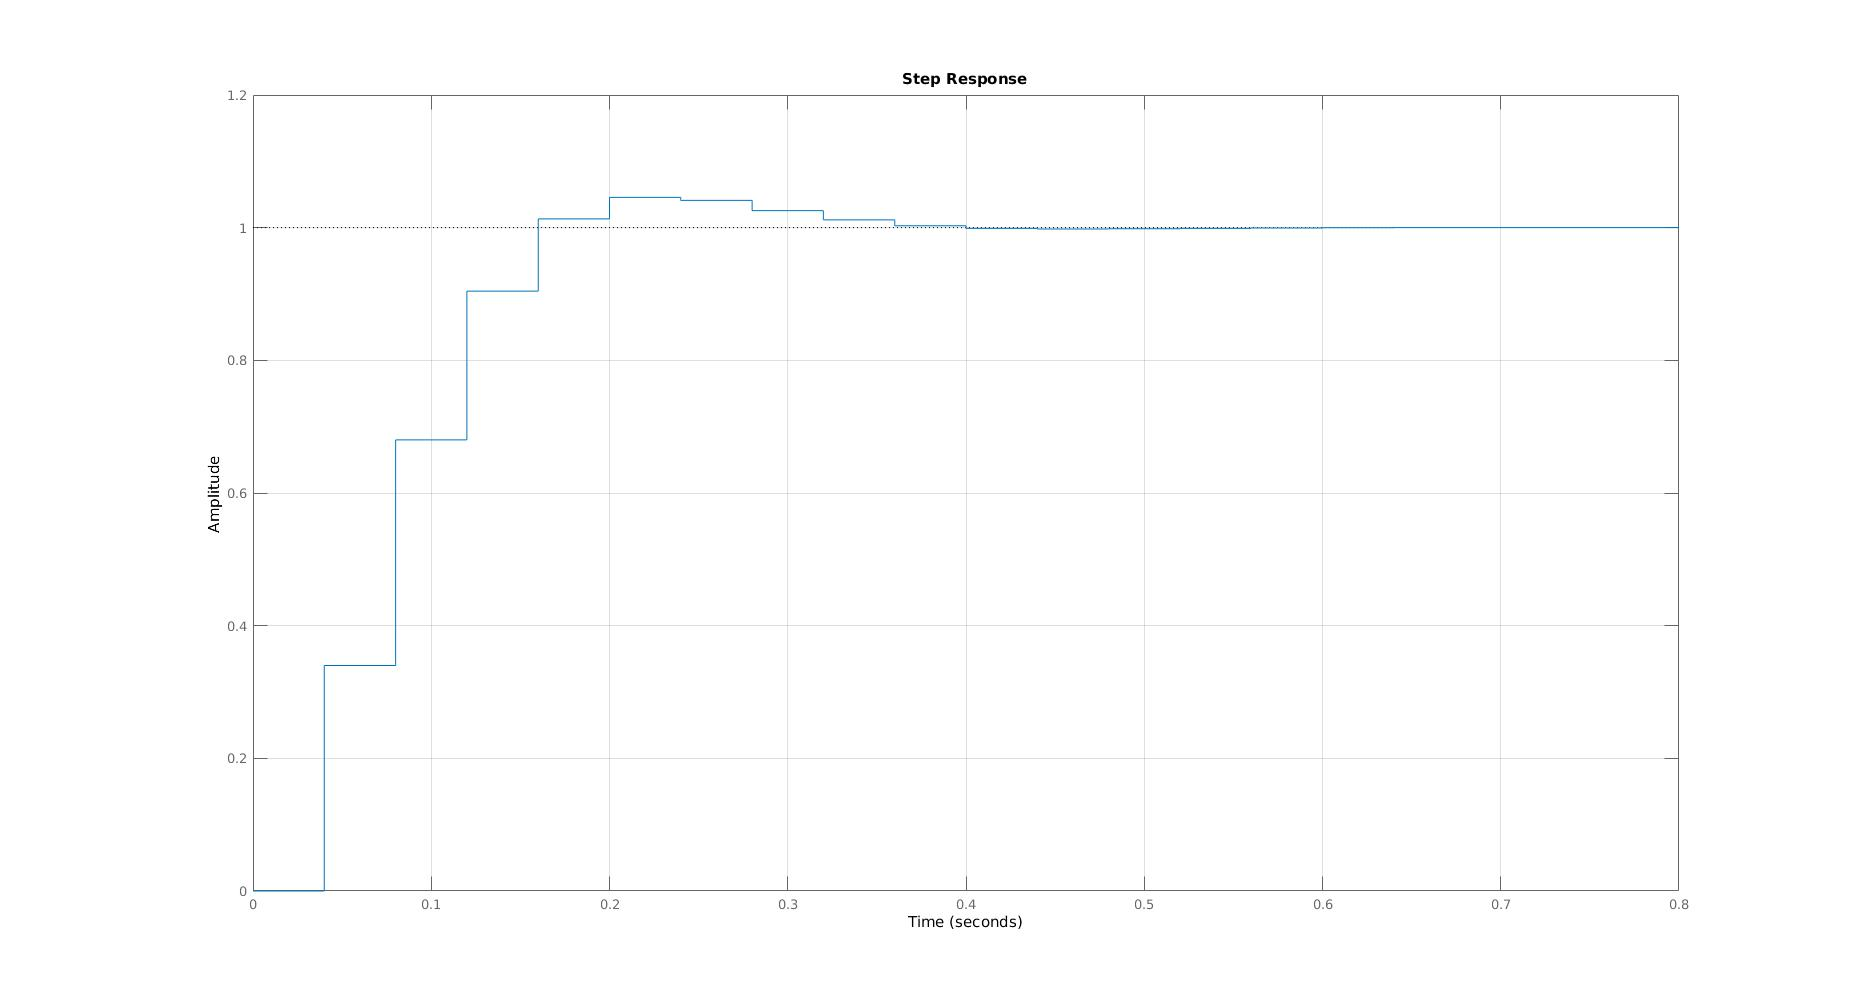
\includegraphics[width=1\linewidth]{Labo3_4_step_response2.jpg}
	\caption{stap responsie van de gesloten lus voor 4\% doorschot}
\end{figure}

In de bovenstaande figuur zien we de stap responsie voor de gesloten lus van het systeem met een doorschot van 4\%. Dit kunnen we zien aan de maximale waarde die deze responsie bereikt, namelijk 1,04.

\subsection{Herhaal de stappen 1 tot en met 3 voor $H(z) = 1/z^2$}
\subsubsection{Stap 1}
\begin{figure}[!h]
	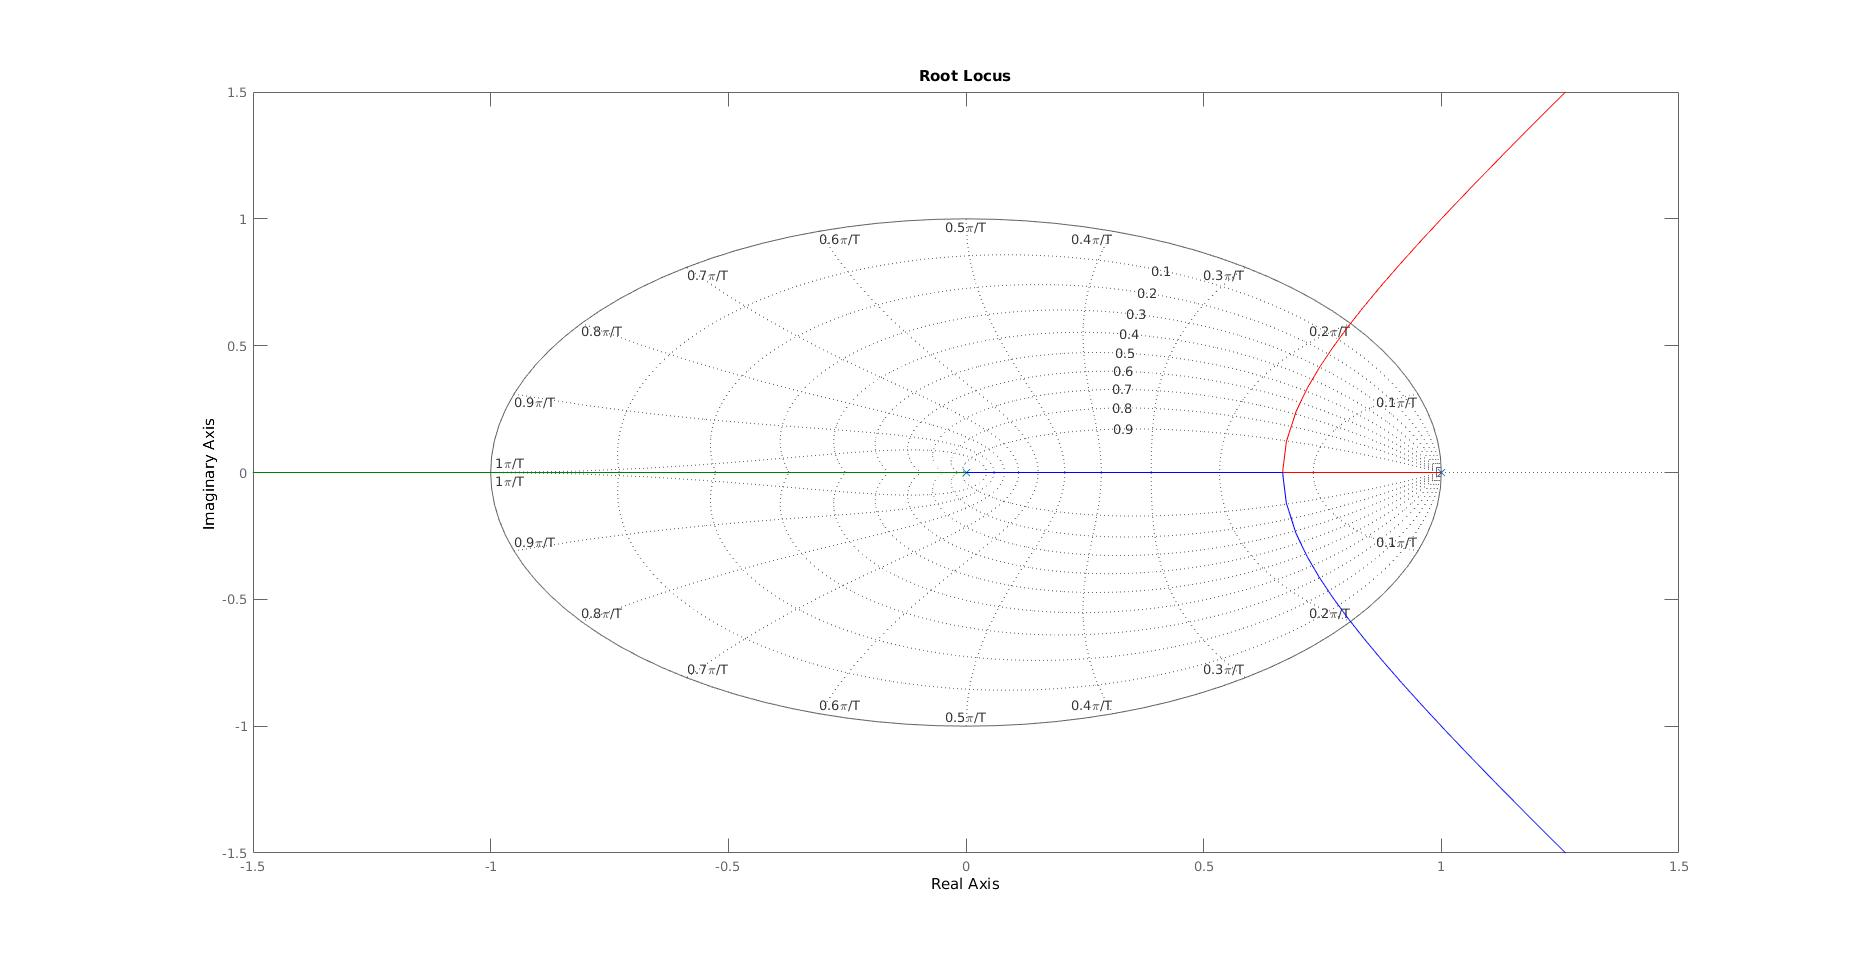
\includegraphics[width=1\linewidth]{Labo3_4_rootlocus3.jpg}
	\caption{nulpunten/polen diagram van de open lus}
\end{figure}

Verder geeft matlab via de functie 'margin()' de versterking om een marginaal stabiel systeem te bekomen. In dit geval is K\textsubscript{marg} = 15,4508.
\subsubsection{Stap 2}

We hebben de figuur bewust ingezoomd omdat de figuur anders niet leesbaar was.

\begin{figure}[!h]
	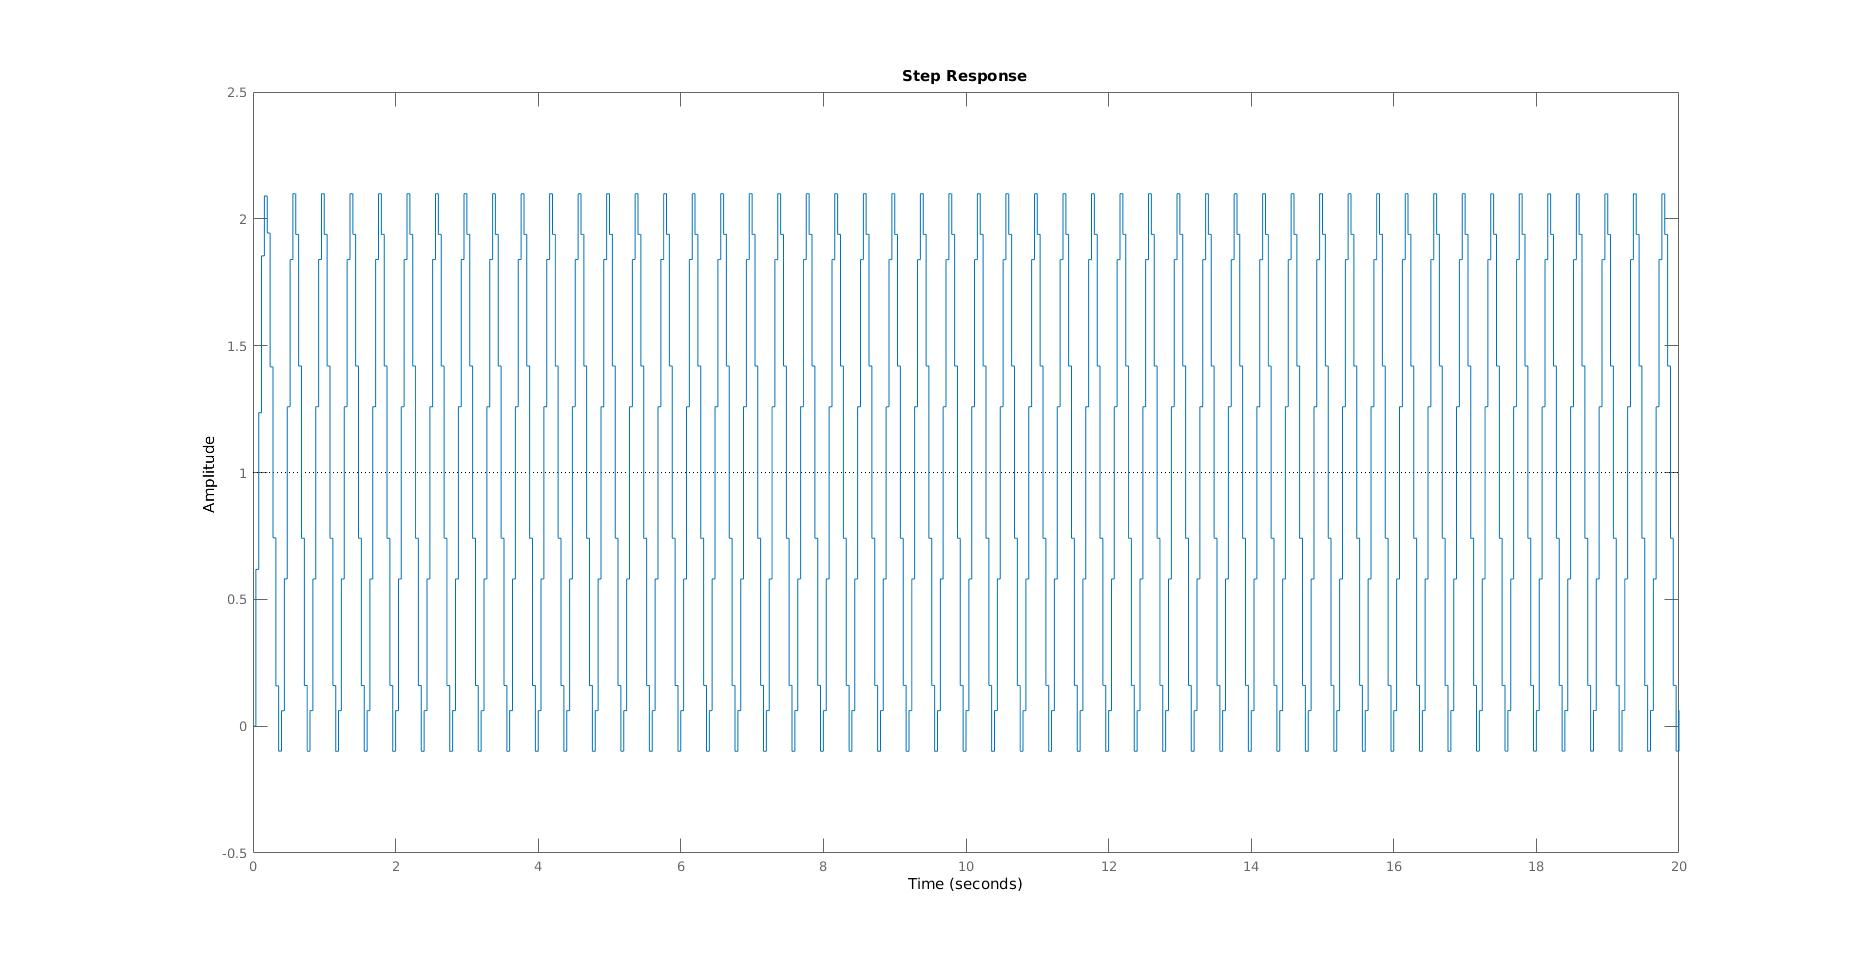
\includegraphics[width=1\linewidth]{Labo3_4_step_response3.jpg}
	\caption{stapresponsie van de gesloten lus met k\textsubscript{marg}}
\end{figure}

\subsubsection{Stap 3}

Voor 4\% doorschot moeten we rekenen met een demping van 0,707.

\begin{figure}[!h]
	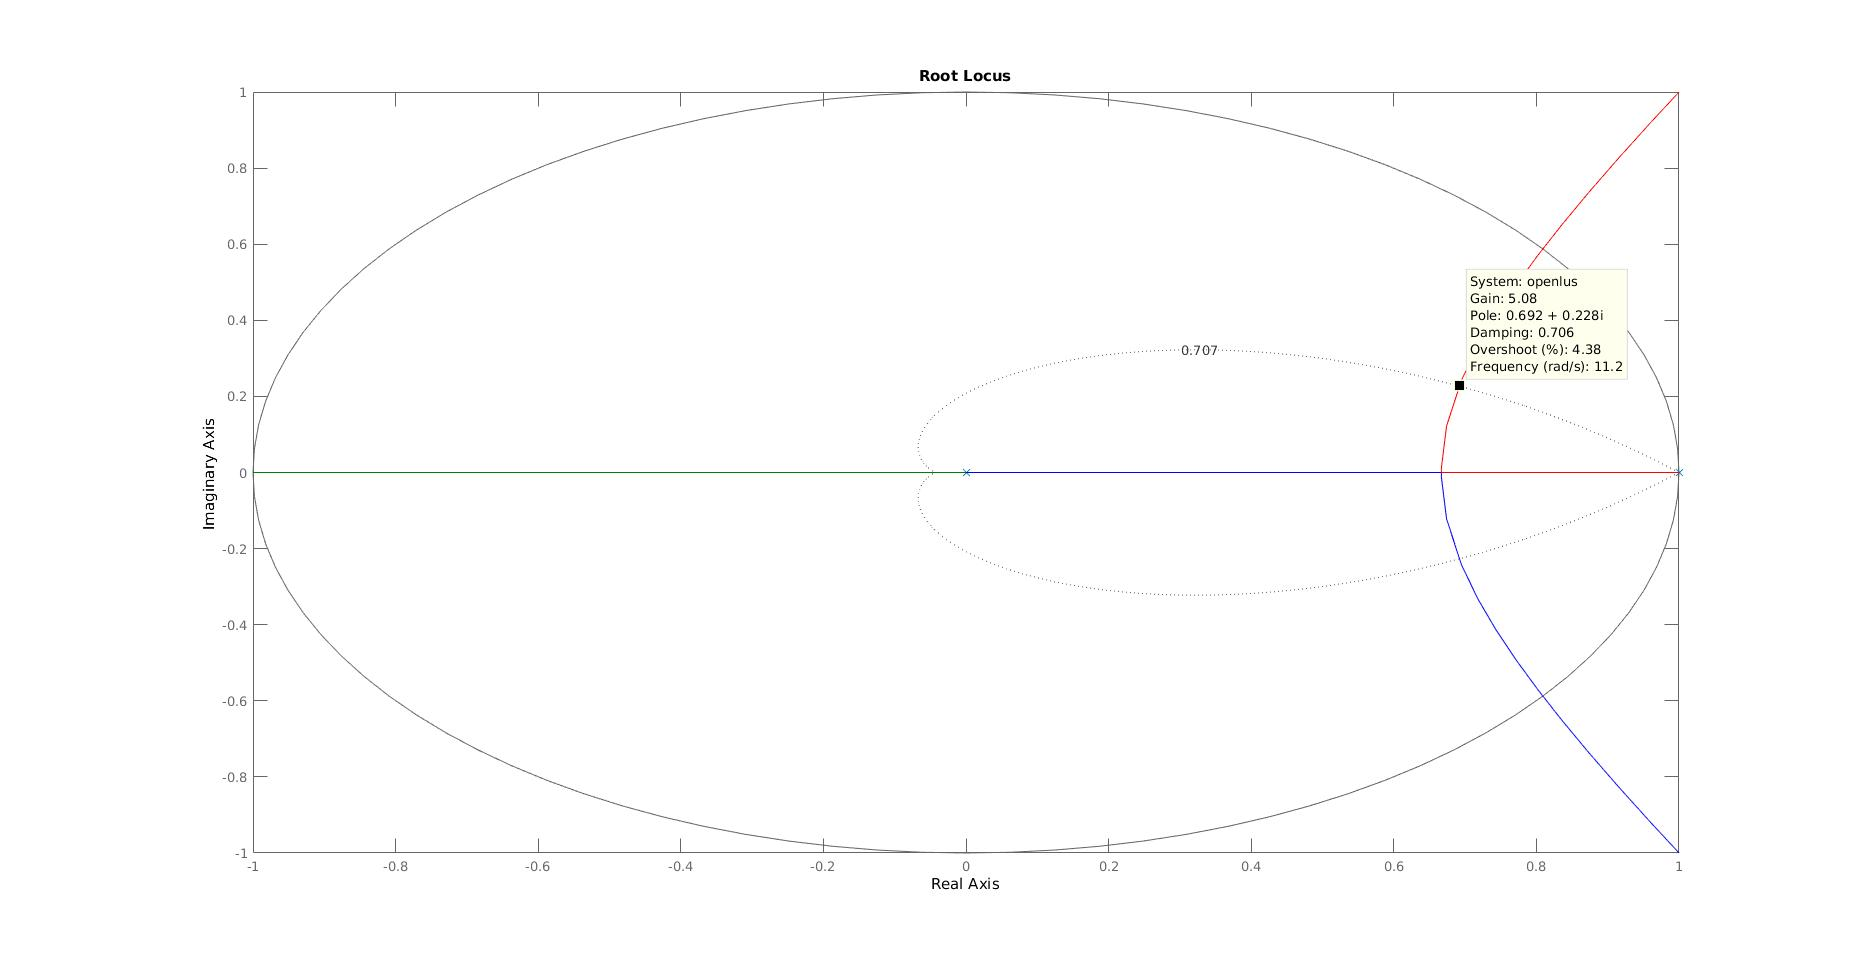
\includegraphics[width=0.9\linewidth]{Labo3_4_rootlocus4.jpg}
	\caption{nulpunten/polen diagram met demping 0,707 aangeduid}
\end{figure}

Uit de figuur kunnen we aflezen dat voor een demping van 0,707 en dus ook doorschot van 4\%, K gelijk is aan 5,08.

\begin{figure}[!h]
	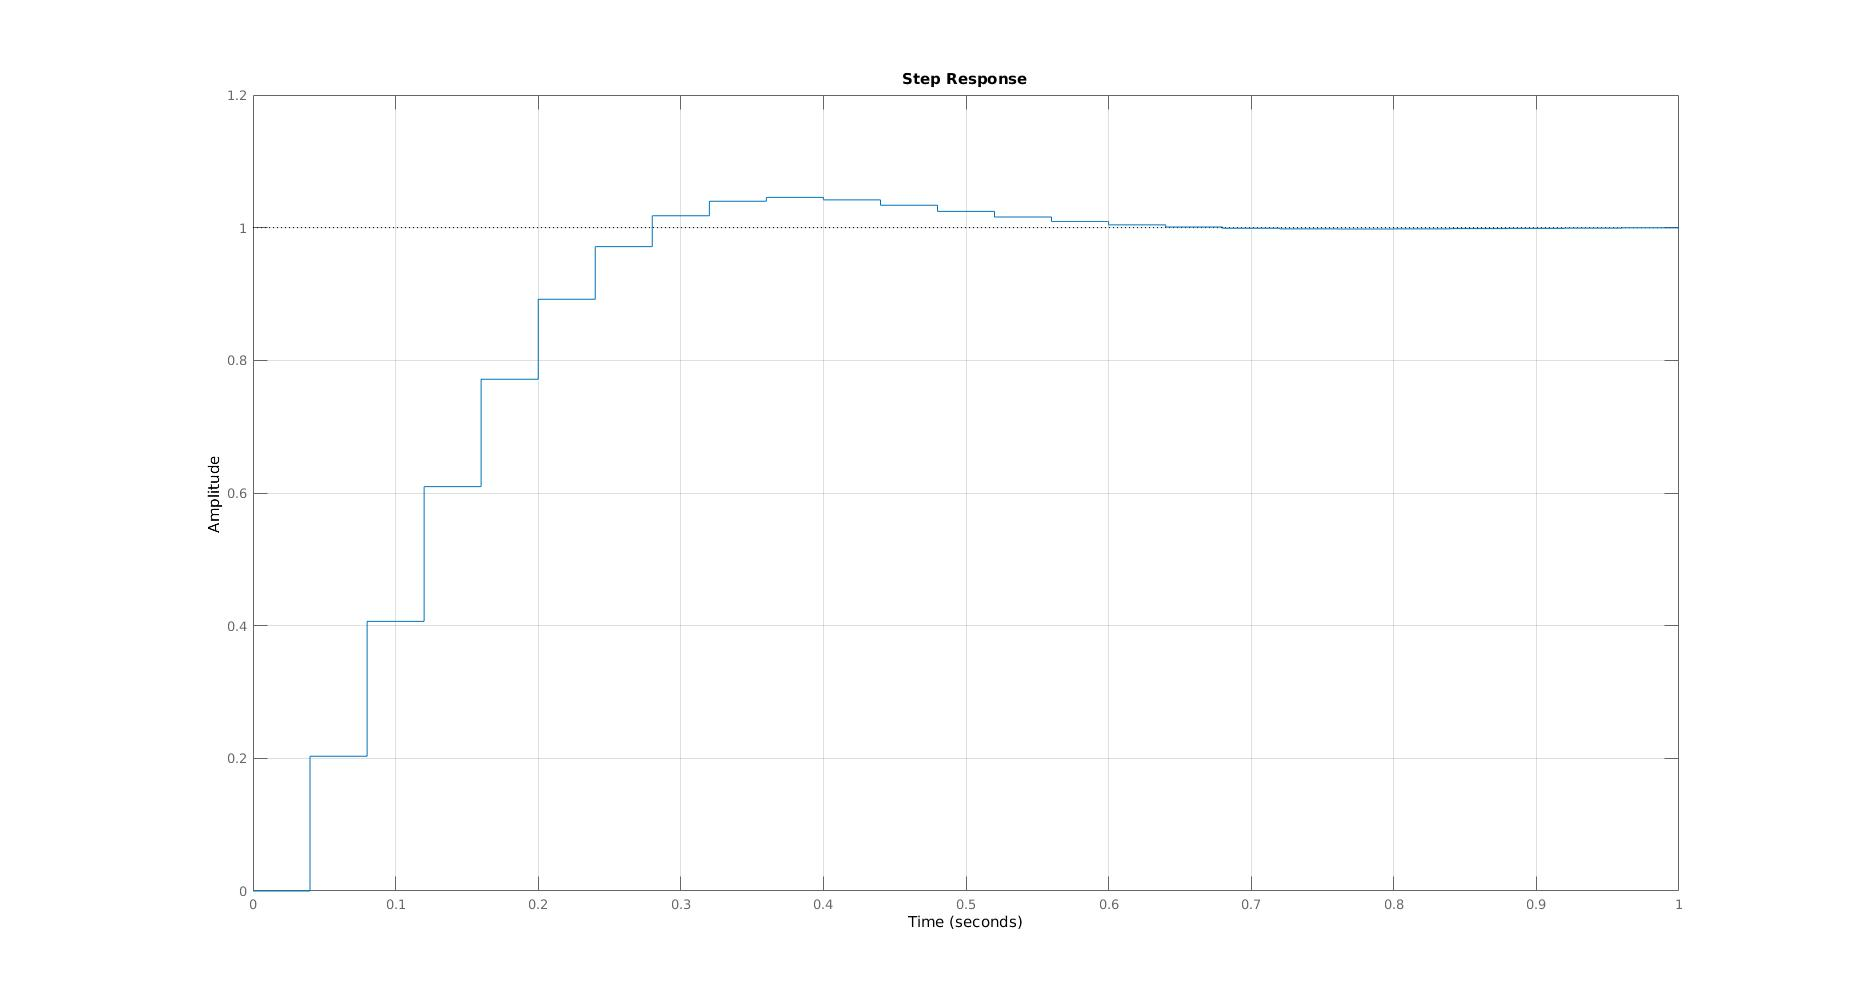
\includegraphics[width=1\linewidth]{Labo3_4_step_response4.jpg}
	\caption{stap responsie van de gesloten lus voor 4\% doorschot}
\end{figure}

In de bovenstaande figuur zien we de stap responsie voor de gesloten lus van het systeem met een doorschot van 4\%. Dit kunnen we zien aan de maximale waarde die deze responsie bereikt, namelijk 1,04.

\section{Simulatie digitale regellus in Simulink}

\begin{figure}[H]
	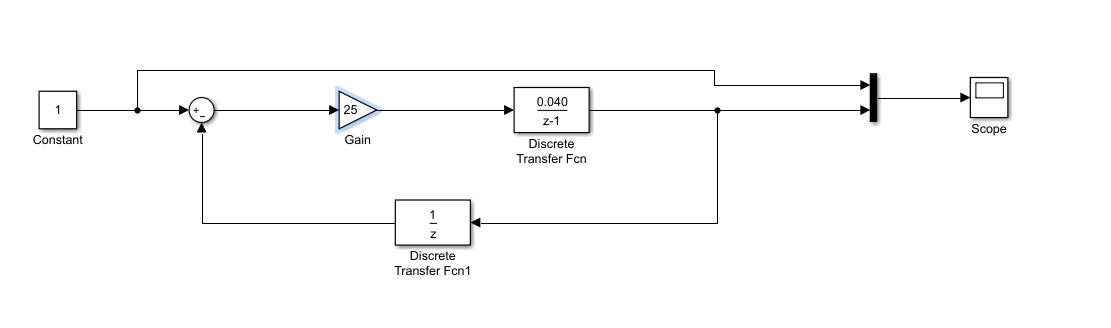
\includegraphics[width=1\linewidth]{Labo3_5_systeem.jpg}
	\caption{schema van de gebruikte regelkring}
\end{figure}

\begin{figure}[H]
	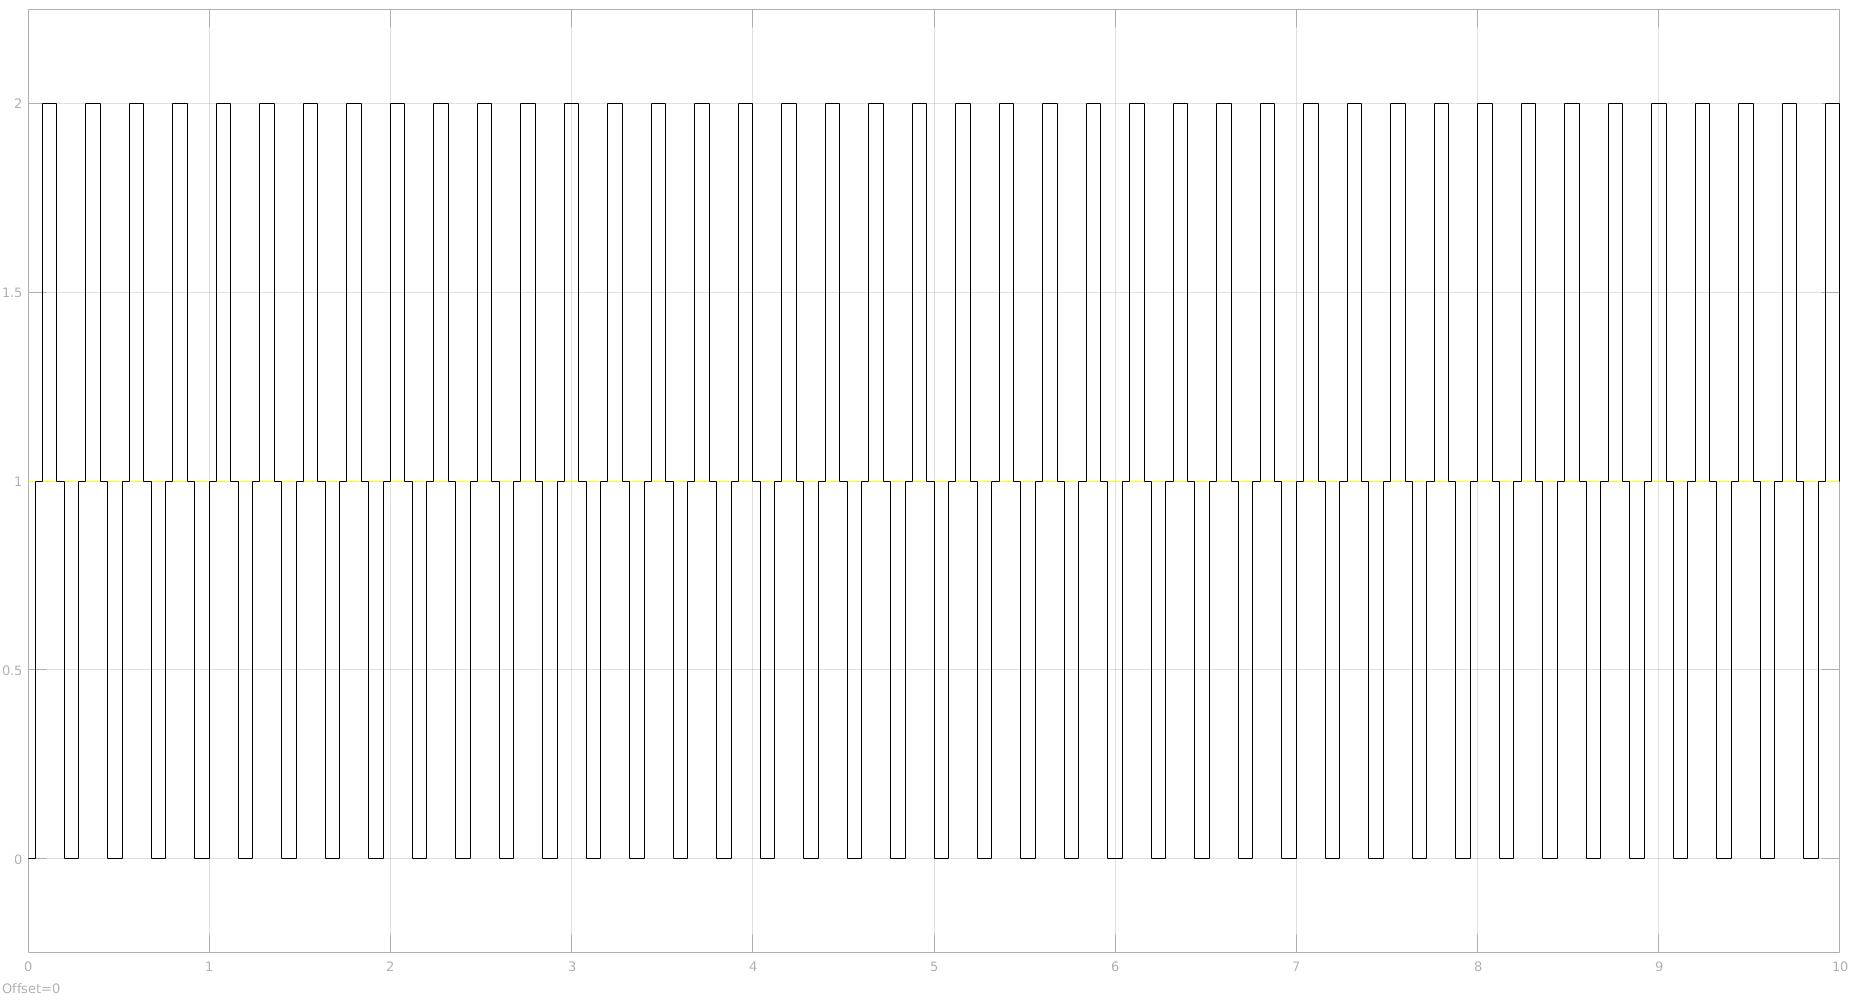
\includegraphics[width=1\linewidth]{Labo3_5_stapresponse.jpg}
	\caption{stap responsie voor een marginaal stabiel systeem}
\end{figure}

\begin{figure}[H]
	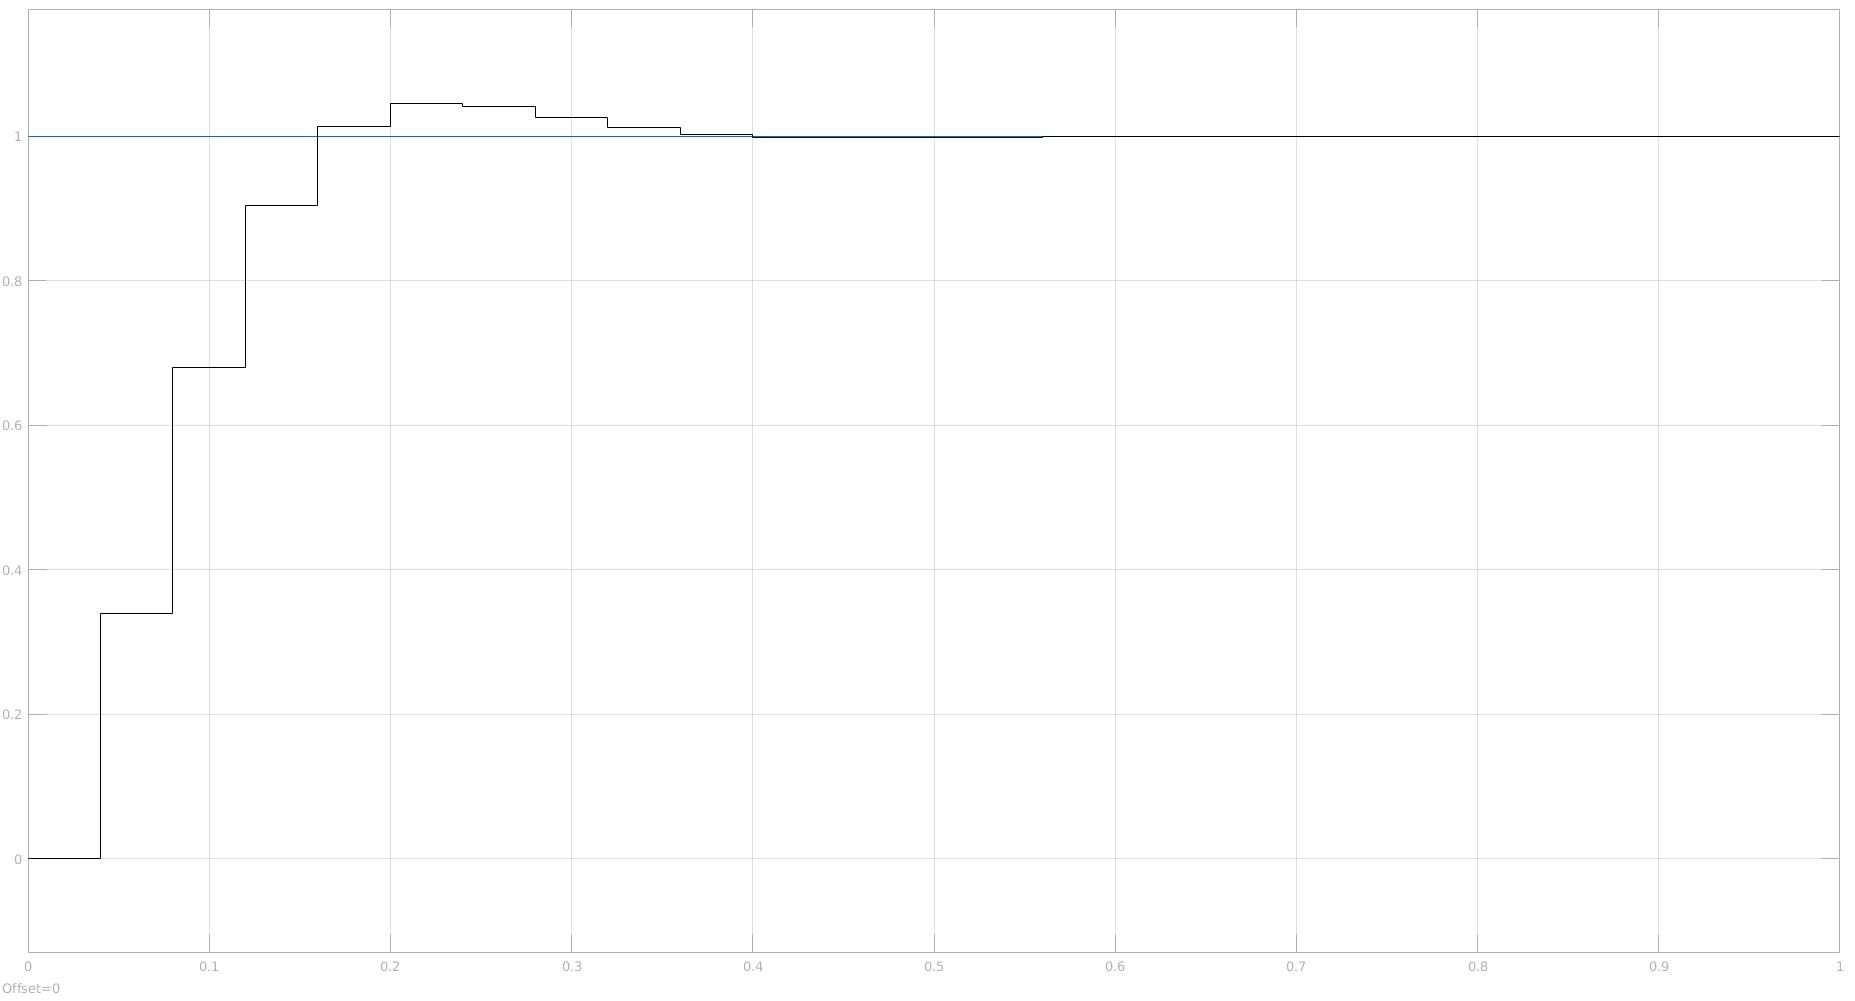
\includegraphics[width=1\linewidth]{Labo3_5_stapresponse2.jpg}
	\caption{stap responsie voor 4\% doorschot}
\end{figure}

\newpage

\section{Bouw eveneens een regellus met een continue integrator als robot-model.}

\begin{figure}[!h]
	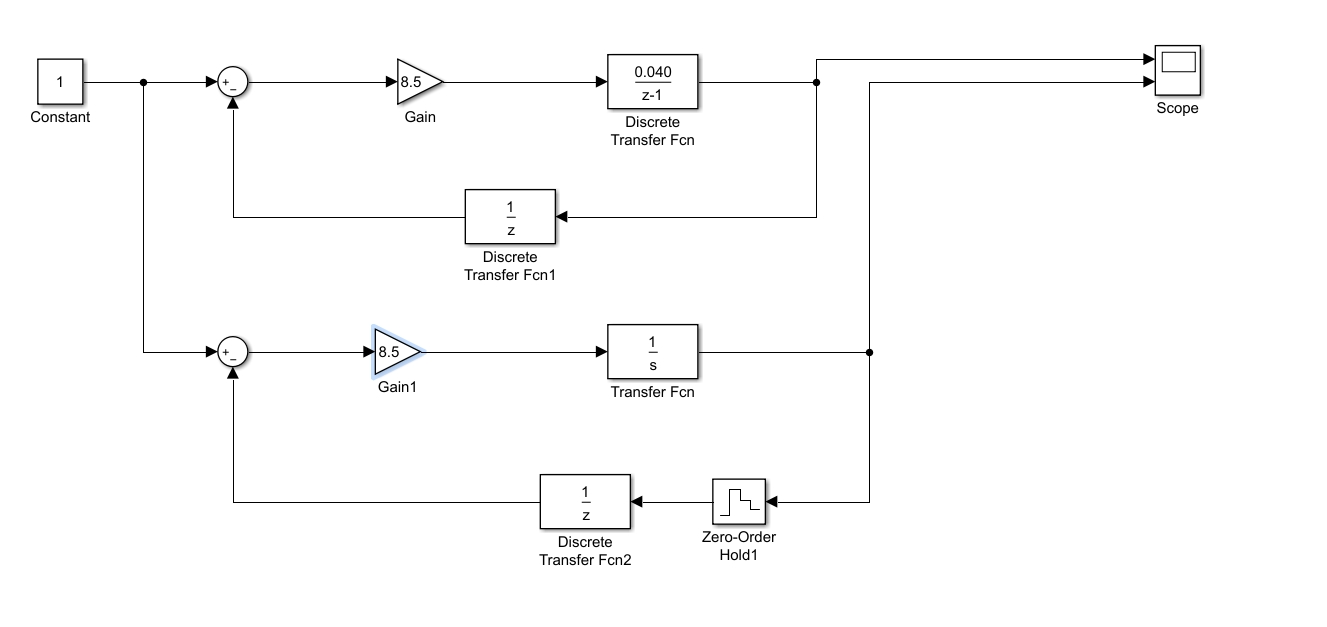
\includegraphics[width=1\linewidth]{Labo3_5_systeem2.jpg}
	\caption{schema van de gebruikte regelkring}
\end{figure}

\begin{figure}[!h]
	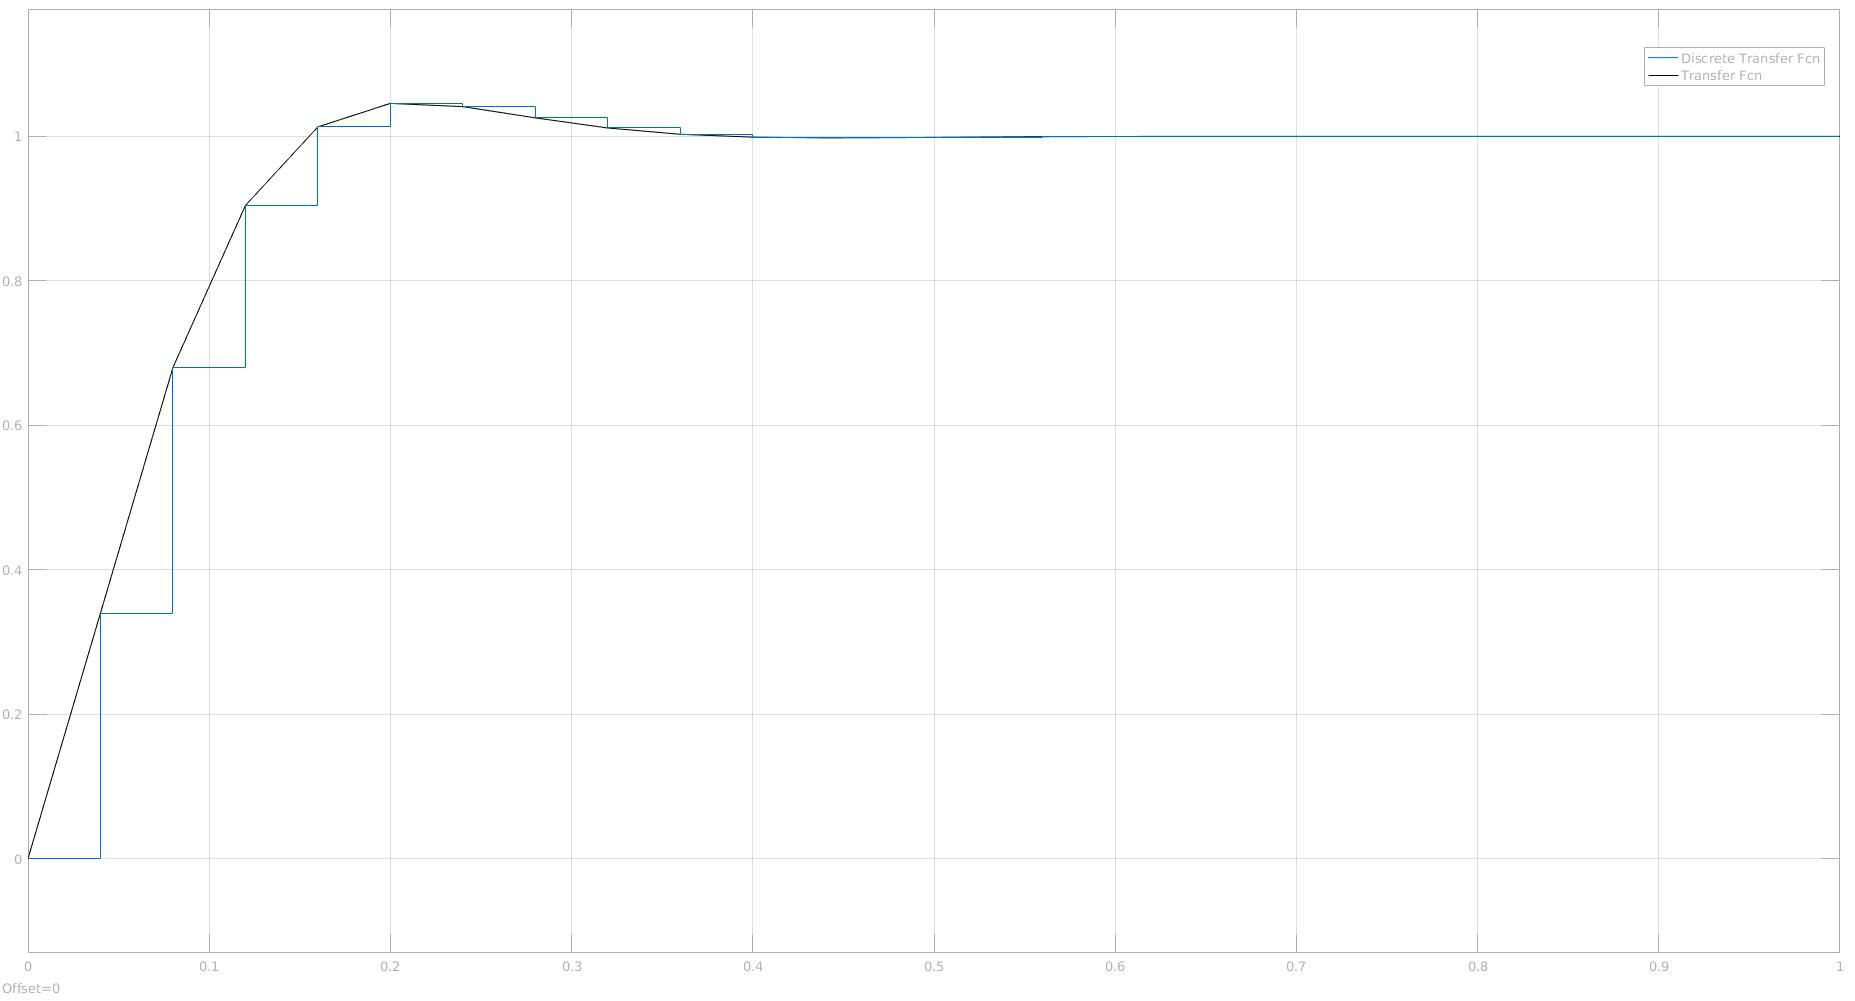
\includegraphics[width=1\linewidth]{Labo3_5_stapresponse3.jpg}
	\caption{stap responsie voor 4\% doorschot}
\end{figure}

We hebben de staprespons voor een marginaal stabiel systeem niet toegevoegd omdat deze onvoldoende duidelijk was. \\

We stellen vast dat als we na het Zero-order-hold blokje meten we het exact hetzelfde signaal krijgen als het discreet equivalent. Als we voor het Zero-order-hold blokje meten krijgen we een continu signaal dat toch het digitaal systeem volgt en per samplemoment een andere richtingscoëfficiënt krijgt.

\section{Gebruik nu een juister robot-model welk bestaat uit een continu eerste orde systeem gevolgd door een continue integrator}

\begin{figure}[!h]
	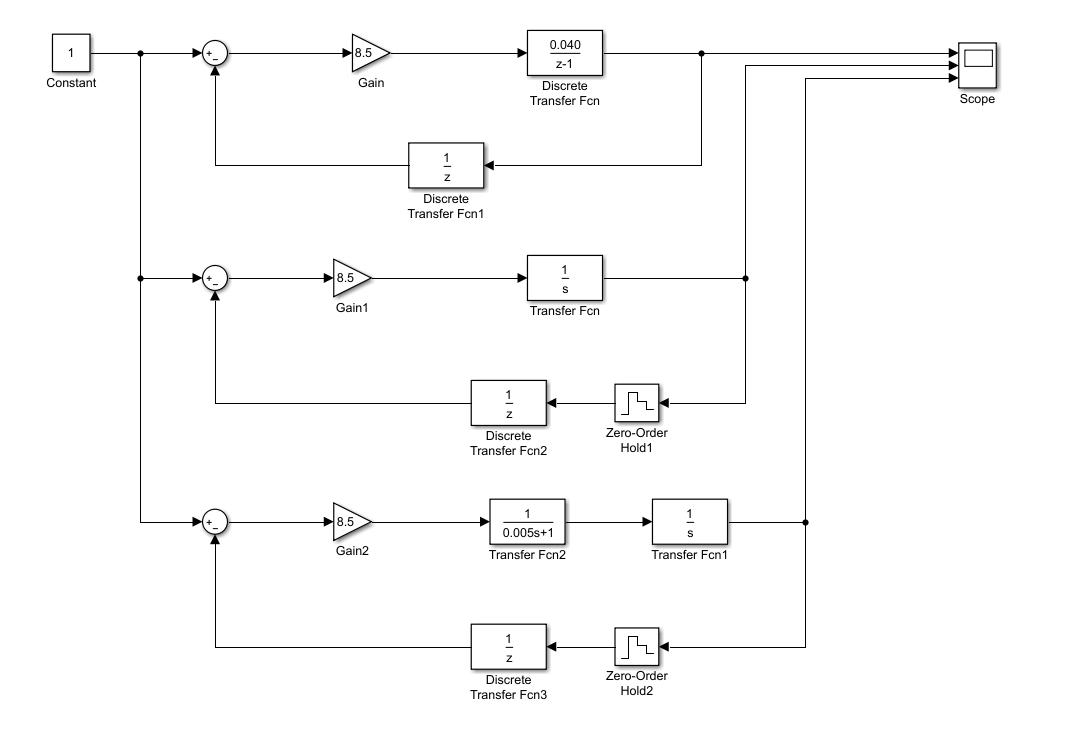
\includegraphics[width=1\linewidth]{Labo3_5_systeem3.jpg}
	\caption{schema van de gebruikte regelkring}
\end{figure}

\begin{figure}[H]
	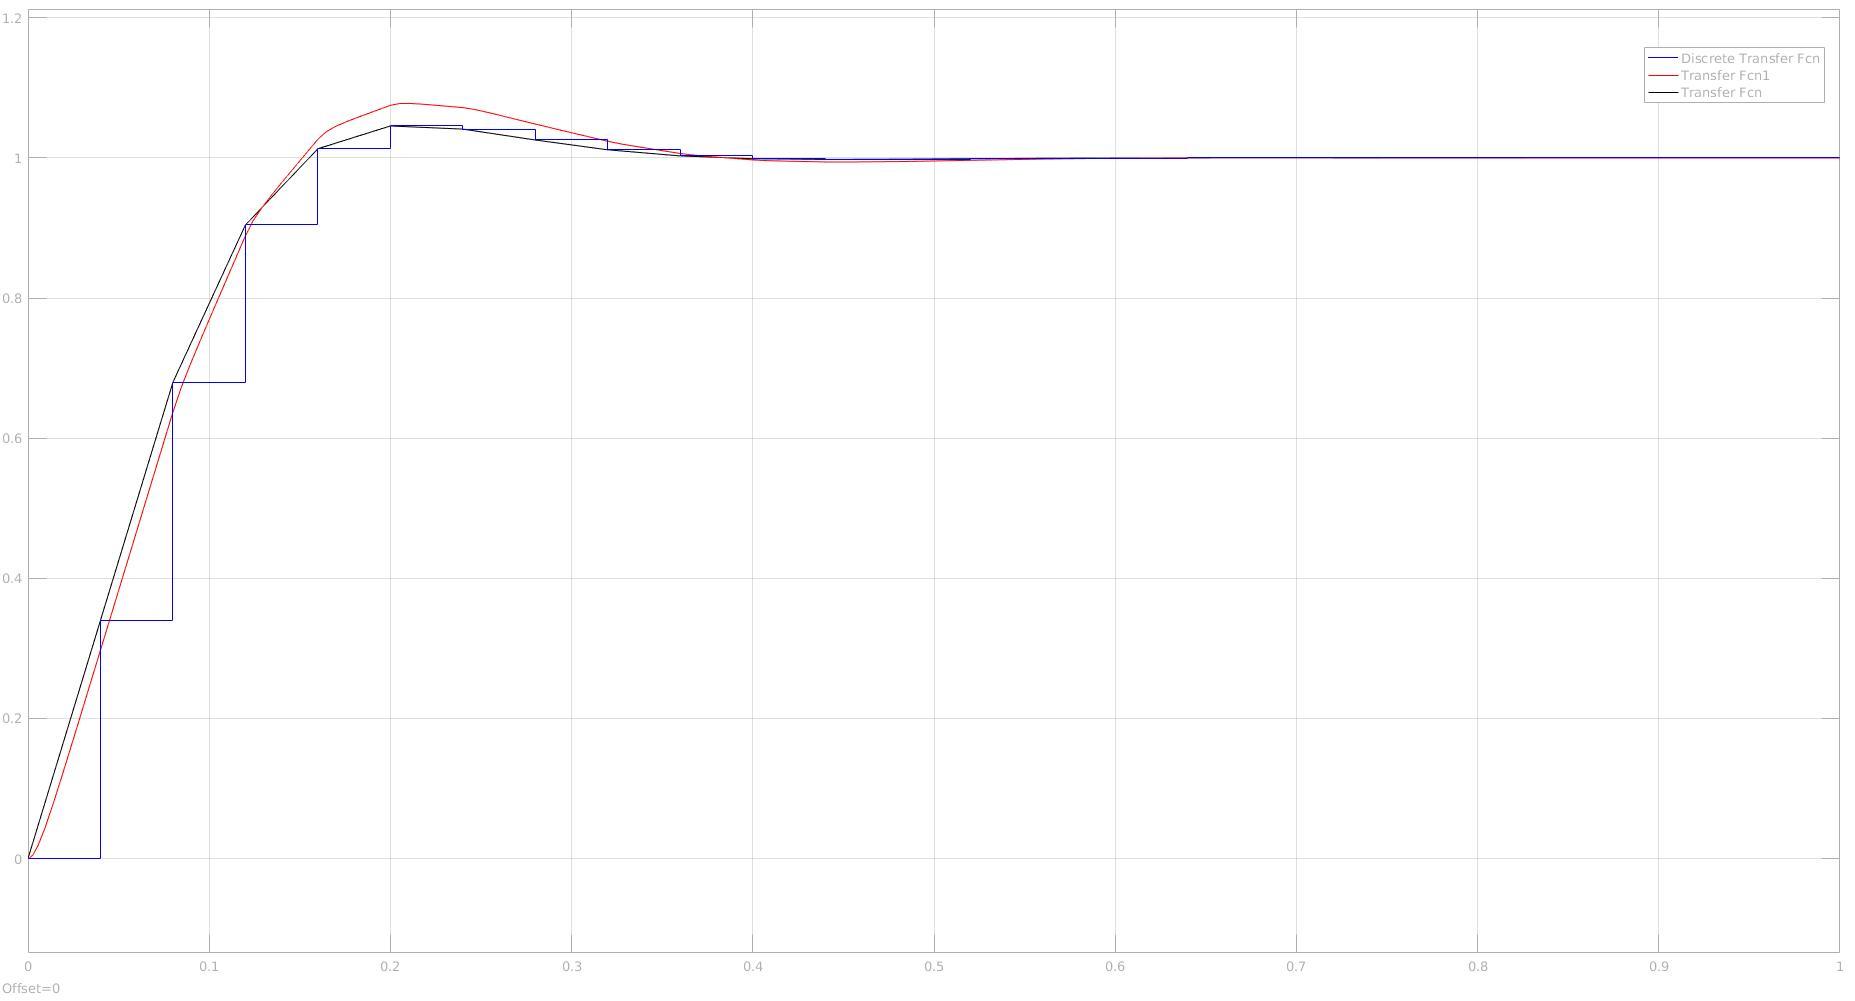
\includegraphics[width=1\linewidth]{Labo3_5_stapresponse4.jpg}
	\caption{stap responsie voor 4\% doorschot}
\end{figure}

In bovenstaande figuur zien we de 3 robot modellen bij elkaar. De eerste 2 hebben we al besproken. De 3de van de robot modellen zou de meest juiste moeten zijn. \\
Toch vertoont het rode model, en dus ook het laatste model meer dan 4\% doorschot. Dit komt mede doordat de de versterking niet voor dit systeem berekend werd.

\end{document}